% !TeX spellcheck = pt_BR
\documentclass[tese_patricia]{subfiles}
\begin{document}
	
\begin{comment}
	\nomenclature[D,01]{$\Omega_{x}$}{Domínio inicial de um sólido deformável;}
	\nomenclature[D,02]{$\lPosition$}{Coordenadas ou posições materiais do domínio inicial;}
	\nomenclature[D,03]{$\Omega_{y}$}{Domínio atual de um sólido deformável;}
	\nomenclature[D,04]{$\ePosition$}{Coordenadas ou posições espaciais do domínio atual;}
	\nomenclature[D,05]{$\deformation$}{Função mudança de configuração para um descrição Lagrangiana;}
	\nomenclature[D,06]{$\greenStrain$}{Tensor de deformações de Green-Lagrange;}
	\nomenclature[D,07]{$\cauchyStretch$}{Tensor de alongamento à direita de Cauchy-Green;}
	\nomenclature[D,08]{$\gradDeformation$}{Grandiente da função mudança de configuração;}
	\nomenclature[D,09]{$\mathbf{u}$}{Vetor qualquer definido na configuração inicial;}
	\nomenclature[D,10]{$\mathbf{v}$}{Vetor qualquer definido na configuração atual;}
	\nomenclature[D,11]{$dV_{0}$}{Infinitésimo de volume definido na configuração inicial;}
	\nomenclature[D,12]{$dV$}{Infinitésimo de81 volume definido na configuração atual;}
	\nomenclature[D,13]{$\mathbf{dx}^{i}$}{Vetor que define o lado $i$ de um infinitésimo de volume na configuração inicial, com $i = 1,2,3$;}
	\nomenclature[D,14]{$dx_{j}^{i}$}{Componente do vetor $mathbf{dx}^{i}$ na direção do eixo $x_{j}$;}
	\nomenclature[D,15]{$\mathbf{dy}^{i}$}{Vetor que define o lado $i$ de um infinitésimo de volume na configuração atual, com $i = 1,2,3$;}
	\nomenclature[D,16]{$dy_{j}^{i}$}{Componente do vetor $mathbf{dy}^{i}$ na direção do eixo $y_{j}$;}
	\nomenclature[D,17]{J}{Jacobiano da transformação, definido como $det(\gradDeformation)$};
	\nomenclature[D,18]{$\mathbf{dA}_{0}$}{Vetor de área da seção transversal de um volume na configuração inicial;}
	\nomenclature[D,19]{$\mathbf{dA}$}{Vetor de área da seção transversal de um volume na configuração atual;}
	\nomenclature[D,20]{$\mathbf{N}$}{Vetor normal a uma superfície na configuração inicial;}
	\nomenclature[D,21]{$\mathbf{n}$}{Vetor normal a uma superfície na configuração atual;}
	\nomenclature[D,22]{${dA}_{0}$}{Área da seção transversal de um volume na configuração inicial;}
	\nomenclature[D,23]{${dA}$}{Área da seção transversal de um volume na configuração atual;}
	\nomenclature[D,24]{$\mathbf{B}$}{Tensor definido como $\mathbf{B} = \gradDeformation^{-t}$;}
	\nomenclature[D,25]{$\extEnergy$}{Energia potencial das forças externas;}
	\nomenclature[D,26]{$\intEnergy$}{Energia de deformação;}
	\nomenclature[D,27]{$\kinEnergy$}{Energia cinética;}
	\nomenclature[D,28]{$\totalEnergy$}{Energia total mecânica;}
	\nomenclature[D,29]{$\delta(\bullet)$}{Variação aplicada a variável $(\bullet)$;}
	\nomenclature[D,30]{$\ebodyLoad$}{Forças de corpo na configuração atual;}
	\nomenclature[D,31]{$\tractionLoad$}{Forças de superfície na configuração atual;}
	\nomenclature[D,32]{$\stressTensor$}{Tensor de tensões de Cauchy;}
	\nomenclature[D,33]{$\rho$}{Massa específica do sólido;}
	\nomenclature[D,34]{$\solidAccel$}{Aceleração do sólido;}
	\nomenclature[D,35]{$\strainratetensor$}{Tensor de deformação linear de engenharia;}
	\nomenclature[D,36]{$M$}{Massa de um corpo;}
	\nomenclature[D,37]{$t$}{Instante de tempo qualquer da análise;}
	\nomenclature[D,38]{$\rho_{0}$}{Massa específica do corpo na configuração inicial;}
	\nomenclature[D,39]{$\ebodyLoad^{0}$}{Forças de corpo na configuração inicial;}
	\nomenclature[D,40]{$\mathbf{P}$}{Tensor de tensões de Piola Kirchhoff;}
	\nomenclature[D,41]{$\tractionLoad^{0}$}{Forças de superfície na configuração inicial;}
	\nomenclature[D,42]{$\piolaStress$}{Segundo tensor de tensões de Piola Kirchhoff;}
	\nomenclature[D,43]{$u_{e}$} {Expressão generalizada da energia de deformação;}
	\nomenclature[D,44]{$\constitutiveTensor$}{Tensor constitutivo elástico isotrópico;}
	\nomenclature[D,45]{$\bulkModulus$}{Módulo volumétrico;}
	\nomenclature[D,46]{$\shearModulus$}{Módulo de cisalhamento;}
	\nomenclature[D,47]{$\elasticModulus$ }{Módulo de elasticidade;}
	\nomenclature[D,48]{$\poisonsRatio$}{Coeficiente de Poisson;}
	\nomenclature[D,49]{$\deformation^{m0}$}{Função mudança de configuração da superfície média de uma casca que mapeia o domínio paramétrico para o domínio inicial;}
	\nomenclature[D,50]{$\lPosition^{m}$}{Posições da superfície média de uma casca na configuração inicial;}
	\nomenclature[D,51]{$\bm{\xi}$}{Coordenadas adimensionais que definem o espaço paramétrico}
	\nomenclature[D,52]{$\mathbf{X}$}{Posições discretas nodais de um elemento de casca na configuração inicial;}
	\nomenclature[D,53]{$N$}{Funções de forma}
	\nomenclature[D,54]{$\deformation^{m1}$}{Função mudança de configuração da superfície média de uma casca que mapeia o domínio paramétrico para o domínio atual;}
	\nomenclature[D,55]{$\ePosition^{m}$}{Posições da superfície média de uma casca na configuração atual;}
	\nomenclature[D,56]{$\SolidPos$}{Posições discretas nodais de um elemento de casca na configuração atual;}
	\nomenclature[D,57]{$\mathbf{v}^{0}$}{Vetor posição definido a partir da superfície média da casca em sua configuração inicial;}
	\nomenclature[D,58]{$\mathbf{v}^{1}$}{Vetor posição definido a partir da superfície média da casca em sua configuração atual;}
	\nomenclature[D,59]{$h_{0}$}{Espessura média inicial de um elemento de casca;}
	\nomenclature[D,60]{$\mathbf{V}^{0}$}{Vetor posição discreto nodal na configuração inicial;}
	\nomenclature[D,61]{$\mathbf{V}^{1}$}{Vetor posição discreto nodal na configuração atual;}
	\nomenclature[D,62]{$\alpha$}{Taxa linear de variação da espessura de um elemento de casca;}
	\nomenclature[D,63]{$\Lambda$}{Taxa linear discreta nodal da variação da espessura de um elemento de casca;}
	\nomenclature[D,64]{$\deformation^{0}$}{Função mudança de configuração de uma casca que mapeia o domínio paramétrico para o domínio inicial;}
	\nomenclature[D,65]{$\deformation^{1}$}{Função mudança de configuração de uma casca que mapeia o domínio paramétrico para o domínio atual;}
	\nomenclature[D,66]{$\mathbf{F}$}{Vetor de forças nodais aplicadas na configuração inicial;}
	\nomenclature[D,67]{$\gradDeformation^{1}$}{Gradiente da função mudança de configuração $\deformation^{1}$;}
	\nomenclature[D,68]{$\gradDeformation^{0}$}{Gradiente da função mudança de configuração $\deformation^{0}$;}
	\nomenclature[D,69]{$\mathbf{B}^{0}$}{Vetor discreto nodal que define as forças de corpo na configuração inicial;}
	\nomenclature[D,70]{$\mathbf{Q}^{0}$}{Vetor discreto nodal que define as forças de superfície na configuração inicial;}
	\nomenclature[D,71]{$\mathbf{\ddot{Y}}$}{Vetor discreto nodal que define a aceleração;}
	\nomenclature[D,72]{$\concLoad^{ext}$}{Vetor discreto nodal que define as forças externas atuantes em um sólido;}
	\nomenclature[D,73]{$\solidMass$}{Matriz de massa de um elemento;}
	\nomenclature[D,74]{$\concLoad^{int}$}{Vetor discreto nodal que define as forças internas atuantes em um sólido;}
	\nomenclature[D,75]{$\solidDamping$}{Matriz de amortecimento de um elemento;}
	\nomenclature[D,76]{$\SolidVel_{}$}{Vetor discreto nodal que define a velocidade;}
	\nomenclature[D,77]{$t_{n+1}$}{Tempo discreto no instante atual;} 
	\nomenclature[D,78]{$t_{n}$}{Tempo discreto no instante anterior;} 
	\nomenclature[D,79]{$\Delta t$}{Intervalo de tempo da discretização temporal;}
	\nomenclature[D,80]{$\beta$}{Parâmetro da aproximação temporal de Newmark;}
	\nomenclature[D,81]{$\gamma$}{Parâmetro da aproximação temporal de Newmark;}
	\nomenclature[D,82]{$\mathbf{Q}_n$ e $\mathbf{R}_n$}{Termos da aproximação de Newmark que relacionam velocidade, aceleração e posições em um instante de tempo anterior;}
	\nomenclature[D,83]{$\NNSS$}{Vetor discreto que representa o resíduo da equação de equilíbrio discretizada no espaço e tempo;}
	
\end{comment}

% ---------------------------------------------------------- 
% Métodos de malhas sobrepostas
% ----------------------------------------------------------
\chapter[Dinâmica dos sólidos computacional]{Dinâmica dos sólidos computacional} \label{capitulo:Cap4}
% ----------------------------------------------------------

Assim como no caso da Mecânica dos Fluidos, um sólido é modelado como um corpo contínuo, com seu movimento governado por um conjunto de equações provenientes da lei da conservação da quantidade de movimento, lei da conservação da massa e lei da conservação de energia. Entretanto, diferentemente dos fluidos, os sólidos possuem resistência aos esforços normais e tangenciais até que alcancem seu limite resistente, e por isso, apresentam deslocamentos e deformações finitos. As variáveis de interesse na resolução do conjunto de equações que descrevem o comportamento do sólido são os deslocamentos, ou, posições atuais ao longo do tempo, dessa forma, uma descrição do tipo Lagrangiana é mais adequada para essas análises.

No contexto da mecânica dos sólidos, o comportamento estrutural pode ser classificado como linear ou não linear. As não linearidades podem ser de natureza geométrica, quando associadas à presença de grandes deslocamentos e rotações que invalidam a hipótese de pequenas deformações, ou de natureza física, quando resultam de modificações na relação constitutiva do material.

Para problemas de sólidos com comportamento elástico, quando houver a possibilidade de grandes deslocamentos, a não-linearidade geométrica deve ser contemplada. Para essa análise, altera-se a forma de consideração do equilíbrio das forças no sólido. Enquanto que em uma modelagem linear, o equilíbrio é realizado em relação a configuração inicial, que é muito próxima a configuração atual do corpo, em uma análise não-linear, o equilíbrio é considerado na configuração atual (ver, por exemplo \citeonline{Ogden:1984} e \citeonline{Coda:2018}).

Em muitos problemas da IFE, como \textit{flutter} e \textit{buffeting}, grandes deslocamentos estão envolvidos. Por isso, nesse estudo, utiliza-se uma formulação não-linear geométrica dinâmica baseada em uma descrição Lagrangiana Total para as análises das estruturas. A formulação é baseada no método dos elementos finitos com abordagem posicional \cite{Coda:2003,Coda:2018}, onde as variáveis principais são as posições nodais. Escolheu-se trabalhar com elementos de cascas, uma vez que esses podem representar a maioria dos problemas estruturais tridimensionais. No casos das cascas, vetores generalizados e um termo que considera a variação linear da espessura do elemento para permitir o mapeamento completo do sólido, são adicionadas às incógnitas nodais do problema. 

Neste capítulo, a formulação é apresentada a partir da descrição da cinemática e das condições de equilíbrio dos corpos deformáveis, com o objetivo de se deduzirem as equações globais de equilíbrio na formulação Lagrangiana, seguida pela introdução do modelo constitutivo de \textit{Saint-Venant–Kirchhoff}. Em seguida, aborda-se o método dos elementos finitos posicional aplicado ao elemento finito de casca, incluindo a técnica de integração temporal empregada. Na sequência, apresenta-se o algoritmo de implementação computacional adotado e, por fim, são expostos os resultados de um exemplo de validação.


\section{Cinemática dos corpos deformáveis}

Um sólido deformável quando sujeito à ações externas, sofre uma mudança de configuração. Na Fig. \ref{fig:solido_cinematica}, pode-se observar um sólido na sua configuração inicial $\Omega_{0}$, com coordenadas materiais descritas por $\lPosition$, e, o sólido no instante atual, representado por $\Omega$, com coordenadas espaciais $\ePosition$. 

\begin{figure}[htb!]
	\centering
	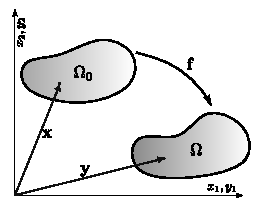
\includegraphics[scale=1.7]{Imagens/Cap4/sol_cinematica.pdf}	
	\caption{Cinemática de um sólido deformável}
	\label{fig:solido_cinematica}
\end{figure}

A função mudança de configuração, denominada de $\fmap$, mapeia cada ponto da posição inicial para a atual, de modo que:

\begin{align}
	\ePosition = \fmap(\lPosition,t).
\end{align}

Uma medida de deformação Lagrangeana deve quantificar a mudança de forma em cada ponto do contínuo em relação ao estado inicial. Para o caso de grandes deslocamentos, assunto desse estudo, a medida de deformação deve ser independente de movimento de corpo rígido ou da escolha dos eixos de referência, ou seja, deve ser uma medida objetiva de deformação. A medida de deformação é descrita em termos do gradiente da função mudança de configuração, $\gradDeformation$, definido matematicamente como:

\begin{align}
	\gradDeformation = \lGrad\left(\fmap\right) = \lGrad\ePosition.
\end{align}

Nesse contexto, o tensor de deformações de Green-Lagrange, respeita a condição de medida de deformação objetiva, sendo descrito de acordo com \citeonline{Ogden:1984} pela seguinte expressão: 

\begin{align}
\greenStrain = \frac{1}{2}\left(\cauchyStretch - \unittensor\right),
\end{align}

\noindent sendo $\cauchyStretch$ um tensor simétrico denominado de tensor de alongamento à direita de Cauchy-Green, o qual é escrito como:

\begin{align}
\cauchyStretch = \gradDeformation^{t} \cdot \gradDeformation =  \gradDeformation \cdot \gradDeformation^{t}.
\end{align}

A partir do gradiente da função mudança de configuração pode-se estabelecer uma relação entre um vetor qualquer $\mathbf{u}$ definido na configuração inicial e seu equivalente na configuração atual $\mathbf{v}$ através da seguinte expressão:

\begin{align}
\mathbf{v} = \gradDeformation \cdot \mathbf{u} \label{eq:rel_vet}
\end{align}

Para a obtenção posteriormente das equações de equilíbrio em descrição Lagrangiana, faz-se necessário abordar as relações de mudança de volume e de área que ocorrem da configuração inicial para a atual. 

No estabelecimento de uma relação entre o volume inicial e final, definem-se dois volumes infinitesimais, um inicial $dV_{0}$ e um final $dV$, apresentados na Fig. \ref{solido_def_vol}. O volume infinitesimal inicial $dV_{0}$ pode ser calculado por:

\begin{align}
dV_{0} = (\mathbf{dx}_{1} \wedge \mathbf{dx}_{2}) \cdot \mathbf{dx}_{3} = \det{(\mathbf{dx_1},\mathbf{dx_2},\mathbf{dx_3})},
\end{align}

\noindent com $\mathbf{dx}_1,\mathbf{dx}_2$ e $\mathbf{dx}_3$ vetores que definem o volume inicial. O volume atual pode ser expresso então, por:

\begin{align}
dV = (\mathbf{dy}_{1} \wedge \mathbf{dy}_{2}) \cdot \mathbf{dy}_{3} = \det{(\mathbf{dy_1},\mathbf{dy_2},\mathbf{dy_3})}, \label{eq:vol_atual}
\end{align}

\noindent  sendo $\mathbf{dy}_1,\mathbf{dy}_2$ e $\mathbf{dy}_3$ os vetores que definem o volume atual.

Tendo em vista a expressão \ref{eq:rel_vet}, pode-se reescrever a Eq. \ref{eq:vol_atual}, como:

\begin{align}
dV = \det{\left(\gradDeformation\right)} \cdot \det{(\mathbf{dx_1},\mathbf{dx_2},\mathbf{dx_3})}  = JdV_{0} \label {eq:vol_atual2},
\end{align}

\noindent na qual $J$ representa o determinante Jacobiano da função mudança de configuração.

\begin{figure}[htb!]
	\centering
	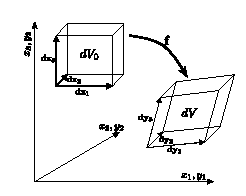
\includegraphics[scale=2.0]{Imagens/Cap4/sol_def_vol.pdf}	
	\caption{Mudança no volume}
	\label{fig:solido_def_vol}
\end{figure}

Para escrever a relação entre as áreas inicial e atual se tomará como referência os cilindros da Fig. \ref{fig:solido_def_area}. Considerando um vetor área inicial $\mathbf{dA}_{0}$ e um vetor área atual $\mathbf{dA}$ como:

\begin{align}
\mathbf{dA}_{0} = \mathbf{N}dA_{0},\\
\mathbf{dA} = \mathbf{n}dA \label{eq:areas},
\end{align}

\noindent com $\mathbf{N}$ e $\mathbf{n}$ os versores unitários normais às áreas inicial $dA_{0}$ e atual $dA$. O volume na configuração inicial ($dV_{0}$) e na configuração atual ($dV$) são calculados por:

\begin{align}
dV_{0} = \mathbf{u} \cdot \mathbf{dA}_{0} = \mathbf{u} \cdot \mathbf{N} dA_0 ,\\
dV = \mathbf{v} \cdot \mathbf{dA} = \mathbf{v} \cdot \mathbf{n} dA \label{eq:vol_func_area},
\end{align}

\noindent com $\mathbf{u}$ e $\mathbf{v}$ vetores não coplanares com as áreas inicial e atual, respectivamente.

\begin{figure}[htb!]
	\centering
	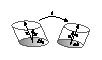
\includegraphics[scale=6.0,trim=0cm 0.2cm 0cm 0cm, clip=true]{Imagens/Cap4/sol_def_area.pdf}	
	\caption{Mudança de área}
	\label{fig:solido_def_area}
\end{figure}

Considerando a relação da Eq. \eqref{eq:rel_vet}, pode-se escrever o volume na configuração atual, $dV$, como:

\begin{align}
	dV = \mathbf{u} \cdot \gradDeformation^{t} \cdot \mathbf{n} dA = J dV_0 = J \mathbf{u} \cdot \mathbf{N} dA_0. \label{eq:dv}
\end{align}

Pré-multiplicando-se a Eq. \refeq{eq:dv} por $\mathbf{B}$ ($(\gradDeformation^{t})^{-1}$) e considerando-se a arbitrariedade de $\mathbf{u}$, chega-se a conhecida fórmula de Nanson, descrita como:

\begin{align}
\mathbf{n}dA = J \mathbf{B} \cdot \mathbf{N} dA_{0}. \label{eq:Nanson}
\end{align}


\section{Equilíbrio de corpos deformáveis} \label{capitulo:Cap3:EquilibrioCorposDeformaveis}

\subsection{Estado de tensão em um ponto}

Um corpo contínuo, ao ser submetido a ações externas, desenvolve forças internas de modo a garantir o equilíbrio dinâmico ou estático. A medida em cada ponto dessas forças internas é fundamental dentro da mecânica dos sólidos para a aplicação das leis da física às partículas do corpo.

Considerando um corpo qualquer, na configuração atual, sujeito a um conjunto equilibrado de forças externas, ao fazer-se a extração de um volume elementar infinitesimal, conforme pode ser observado na Fig. \ref{fig:sol_equi}, surgem em suas faces, por ação e reação, uma distribuição de forças por unidade de superfície. Decompondo essas tensões em componentes cartesianas, obtém-se em cada face uma componente normal e duas componentes tangenciais de tensão. As componentes de tensão são designadas por $\sigma_{ij}$, com $i$ referindo-se ao plano de atuação e $j$ indicando a direção de atuação da tensão. Na Fig. \ref{fig:sol_equi} podem ser observadas as componentes positivas de tensão em cada plano. No plano paralelo oposto, pela lei da ação e reação, as tensões possuem mesma intensidade, porém sentido contrário.

\begin{figure}[htb!]
	\centering
	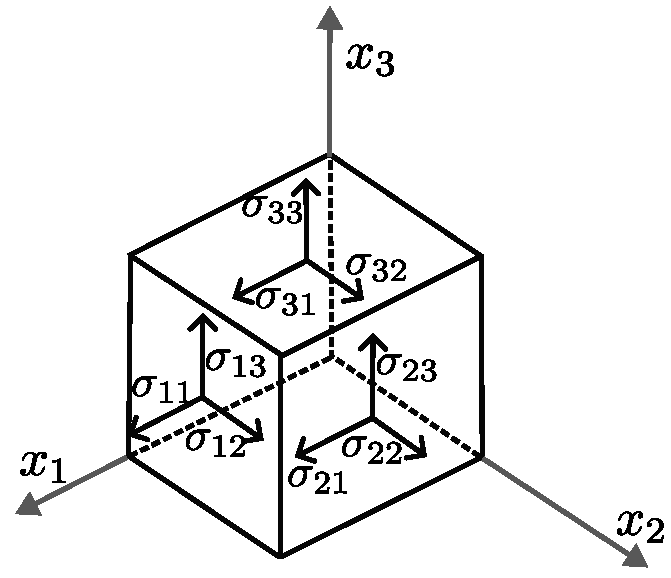
\includegraphics[scale=0.5,trim=0cm 0.0cm 0cm 0cm, clip=true]{Imagens/Cap4/sol_vol_equi.pdf}	
	\caption{Volume infinitesimal: componentes de tensão}
	\label{fig:sol_equi}
\end{figure}

O tensor de tensões de Cauchy ($\cauchyStress$) contém todas as informações de tensão em um ponto e será representado como:

\begin{align}
\cauchyStress =
\begin{bmatrix}
	\sigma_{11} & \sigma_{12} & \sigma_{13} \\
	\sigma_{21} & \sigma_{22} & \sigma_{23} \\
	\sigma_{31} & \sigma_{32} & \sigma_{33}
\end{bmatrix}
.
\end{align}

Ao realizar-se o equilíbrio de momentos sobre um elemento infinitesimal, nota-se que $\cauchyStress$ é simétrico (Teorema de Cauchy), e pode ser reescrito como:

\begin{align}
	\cauchyStress =
	\begin{bmatrix}
		\sigma_{11} & \sigma_{12} & \sigma_{13} \\
		\sigma_{12} & \sigma_{22} & \sigma_{23} \\
		\sigma_{13} & \sigma_{23} & \sigma_{33}
	\end{bmatrix}
	.
\end{align}

Vale ressaltar que, a tensão de Cauchy é definida na configuração atual do contínuo, e por isso, trata-se de uma medida Euleriana de tensão.

Se extraíssemos do corpo contínuo um volume tetraédrico (Fig. \ref{fig:sol_tetra}), no plano inclinado, cujo versor normal é $\mathbf{n}$, surge um vetor de tensões designado por $\mathbf{t}$. Considerando que a área do plano inclinado foi definida como $dA$, enquanto que as áreas correspondentes aos planos coordenados são suas projeções, pode-se calcular o equilíbrio do tetraedro em cada direção, chegando-se a seguinte expressão:

\begin{align}
	\mathbf{t} = \cauchyStress^{t} \cdot \mathbf{n} =  \cauchyStress \cdot \mathbf{n}.
\end{align}

\begin{figure}[htb!]
	\centering
	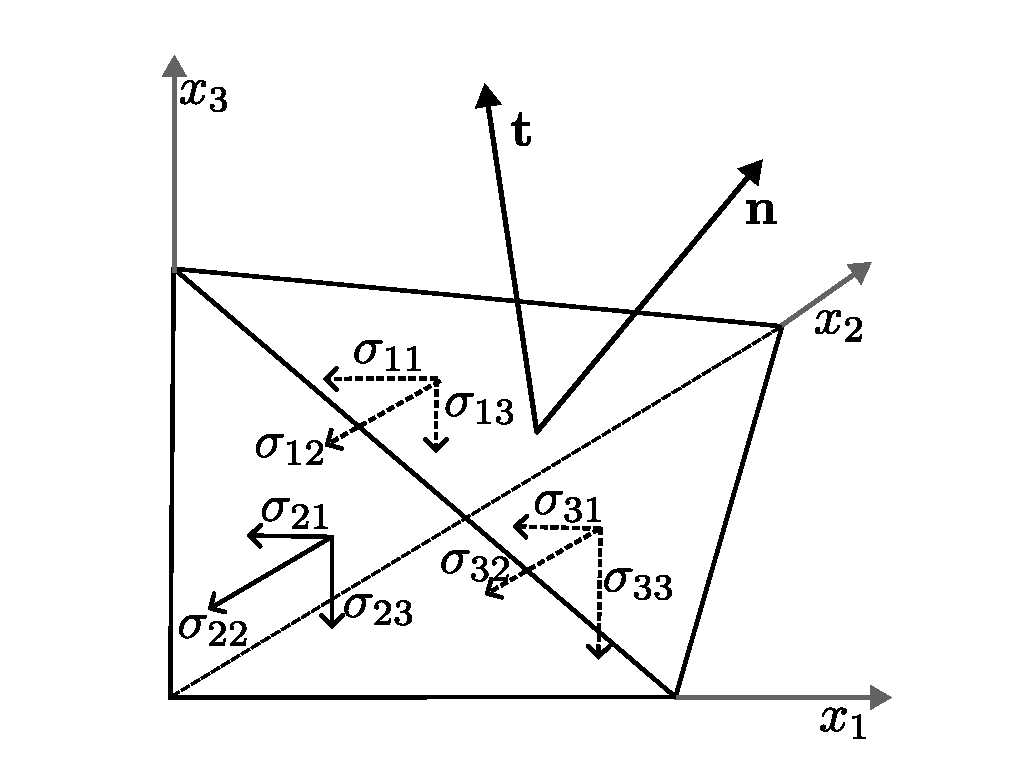
\includegraphics[scale=0.5,,trim=0cm 0.0cm 0cm 0cm, clip=true]{Imagens/Cap4/sol_tetra_equi.pdf}	
	\caption{Tetraedro elementar}
	\label{fig:sol_tetra}
\end{figure}

Essa expressão é conhecida por fórmula de Cauchy. Considerando que o plano inclinado refere-se a superfície externa, essa equação pode ser utilizada para relacionar o estado de tensão em um ponto com as forças de superfície ($\mathbf{p}$), como:
 
\begin{align}
	\mathbf{p} = \cauchyStress^{t} \cdot \mathbf{n} =  \cauchyStress \cdot \mathbf{n}.
\end{align}


\subsection{Equilíbrio local Lagrangeano}

Para a obtenção das equações de equilíbrio local em descrição Lagrangeana, será utilizada como ponto de partida a equação de equilíbrio local Euleriana. Para isso, considere o sólido apresentado na Fig. \ref{fig:sol_cargas}, o qual está submetido a forças de corpo, $\ebodyLoad$, e a forças de superfície, $\tractionLoad$. Extraindo-se um elemento infinitesimal deste corpo que sofreu mudança de configuração, e aplicando-se a segunda Lei de Newton, o  equilíbrio local pode ser descrito:

\begin{align}
	\gradient \cdot \stressTensor^{t} + \ebodyLoad = \rho  \solidAccel, \label{eq:equi_local_euleriano}
\end{align}

\noindent ou ainda, em notação indicial:

\begin{align}
	\sigma_{ji,j} + b_i  = \rho  \ddot{y_i},
\end{align}

\noindent com $\rho$ representando a massa específica do material que compõe o sólido e $\solidAccel$ é a derivada material da velocidade do ponto material (aceleração do corpo).

\begin{figure}[htb!]
	\centering
	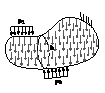
\includegraphics[scale=4,trim=0cm 0.0cm 0cm 0cm, clip=true]{Imagens/Cap4/sol_cargas.pdf}	
	\caption{Sólido sujeito a um conjunto de carregamento externo}
	\label{fig:sol_cargas}
\end{figure}

Ao integrar-se a Eq. \ref{eq:equi_local_euleriano} no volume do sólido e utilizar-se o Teorema da Divergência chega-se a:

\begin{align}
	\int_{A} {\stressTensor}^{t} \cdot \mathbf{n} dA + \int_{V} \ebodyLoad dV = \int_{V} \rho  \solidAccel dV \label{eq:eq_global_euleriano}
\end{align}

\noindent ou, ainda:

\begin{align}
	\int_{A} \mathbf{p} dA + \int_{V} \ebodyLoad dV = \int_{V} \rho  \solidAccel dV 
\end{align}

Considerando as relações de mudança de área e volume, apresentadas nas equações Eq. \ref{eq:vol_atual2} e Eq. \ref{eq:Nanson}, e que da equação da conservação da massa ($M$) tem-se que:

\begin{align}
	M = \int_{V_{0}} \rho_{0}dV_{0} = \int_{V(t)} \rho(t)dV, \label{eq:conser_massa}
\end{align}

\noindent escreve-se a equação global de equilíbrio Lagrangeana, a partir da Eq. \ref{eq:eq_global_euleriano} como:

\begin{align}
	\int_{A_0} \mathbf{P}^t \cdot \mathbf{N} dA_0 + \int_{V_0} \bodyLoad dV_0 = \int_{V_0} \rho_0  \solidAccel dV_0, \label{eq:equi_global_lagrangeano}
\end{align}

\noindent na qual o primeiro tensor de tensões transposto de Piola-Kirchhoff ($\mathbf{P}^t$), não simétrico, é definido como $\mathbf{P}^t = J \stressTensor^t \cdot \mathbf{B}$, e o subíndice $0$, refere-se a variável no instante inicial.

Ao aplicar-se o Teorema da Divergência a Eq. \ref{eq:equi_global_lagrangeano} e da consideração da arbitrariedade do volume, chega-se a versão local da equação de equilíbrio Lagrangeano, expressa por:

\begin{align}
	\lGrad \cdot \mathbf{P}^t +  \bodyLoad = \rho_0  \solidAccel. \label{eq:equi_local_lagrangeano}
\end{align}


\subsection{Princípio de Estacionariedade de energia}

No estudo do equilíbrio de corpos deformáveis a análise da energia mecânica é um assunto de grande importância. A energia mecânica é formada basicamente por três parcelas: energia potencial das forças externas ($\extEnergy$), energia de deformação ($\intEnergy$) e energia cinética ($\kinEnergy$). A energia total mecânica ($\totalEnergy$) é um funcional obtido pela soma dessas três parcelas, sendo escrita da seguinte maneira:

\begin{align}
	\totalEnergy = \extEnergy + \kinEnergy + \intEnergy.
\end{align}

O princípio da estacionariedade da energia define que um corpo quando em equilíbrio apresenta a primeira variação do funcional de energia mecânica nula, sendo o equilíbrio estável quando a posição de equilíbrio representa um mínimo local para a energia mecânica total. Este princípio, para uma descrição das equações de equilíbrio em posições, pode ser expresso matematicamente da seguinte forma:

\begin{align}
	\delta\totalEnergy = \frac{\partial{\totalEnergy}}{\partial{\ePosition}} \cdot \delta\ePosition = \mathbf{0}, \label{eq:princ_esta}
\end{align}

\noindent ou, dada a arbitrariedade de $\delta\ePosition$, como: 

\begin{align}
	\delta\totalEnergy = \delta\extEnergy + \delta\kinEnergy + \delta\intEnergy.
\end{align}

Um incremento de energia mecânica específica (energia mecânica por unidade de volume) pode ser obtido pelo produto escalar da Eq. \ref{eq:equi_local_lagrangeano} por um incremento de posição $\delta\ePosition$, e, integrando-se sobre o domínio inicial, têm-se:

\begin{align}
	\delta\totalEnergy = \int_{V_0} \left(\rho_0 \solidAccel - \lGrad \cdot \mathbf{P}^t -  \ebodyLoad_0 \right) \cdot  \delta\ePosition dV_0 = 0 \label{eq:equi_local_forma_frac}
\end{align}

Ao integrar-se por partes o segundo termo da Eq. \ref{eq:equi_local_forma_frac} e utilizar-se o Teorema da Divergência, chega-se a seguinte expressão:

\begin{align}
	\delta\totalEnergy = \int_{V_0} \rho_0 \solidAccel \cdot \delta\ePosition dV_0 - \int_{A_0} \mathbf{P}^t \cdot \mathbf{N} \cdot  \delta\ePosition dA_0  + \int_{V_0} \mathbf{P}^t : \lGrad(\delta\ePosition) dV_0 - \int_{V_0} \mathbf{b_0} \cdot \delta \ePosition dV_0 = 0 \label{eq:equi_local_forma_frac2}
\end{align}

A equação Eq. \ref {eq:equi_local_forma_frac2} pode ainda ser reformulada, considerando que $\lGrad (\delta\ePosition) = \delta \gradDeformation$ e que $\mathbf{P}^t \cdot \mathbf{N}$ representa as forças de superfície na configuração inicial ($\ltractionLoad$) como:

\begin{align}
\delta\totalEnergy = \int_{V_{0}} \rho_{0} \solidAccel \cdot \delta\ePosition dV_{0} - \int_{A_{0}} \ltractionLoad \cdot \delta\ePosition dA_{0} + \int_{V_{0}} \mathbf{P}^{t} : \delta\gradDeformation dV_{0} - \int_{V_{0}}  \bodyLoad \cdot \delta\ePosition dV_{0} = 0. \label{eq:equi_local_forma_frac3}
\end{align}

Conforme relatou-se, o tensor de Piola-Kirchhoff de primeira espécie não é necessariamente simétrico, desta forma, torna-se mais conveniente adotar uma medida de tensão que resulte em um tensor simétrico. Com essa finalidade, adota-se um tensor $\piolaStress$, de forma que:

\begin{align}
\mathbf{P} = \piolaStress^{t} \cdot \gradDeformation^{t}, \label{eq:piola-kircchoff}
\end{align}

\noindent com $\piolaStress$ conhecido como tensor de Piola-Kirchhoff de segunda espécie. 

Utilizando-se a relação apresentada na Eq. \ref{eq:piola-kircchoff} na Eq. \ref{eq:equi_local_forma_frac3}, chega-se a:

\begin{align}
\delta\totalEnergy = \int_{V_{0}} \rho_{0} \solidAccel \cdot \delta\ePosition dV_{0} - \int_{A_{0}} \ltractionLoad \cdot \delta\ePosition dA_{0} +  \int_{V_{0}} \piolaStress : \delta\greenStrain dV_{0} - \int_{V_{0}}  \bodyLoad \cdot \delta\ePosition dV_{0} = 0.
\label{eq:equi_local_forma_final}
\end{align}

Partindo-se da Eq. \ref{eq:equi_local_forma_final}, encontra-se a relação entre suas componentes e as parcelas de energia mecânica, dessa forma, têm-se:

\begin{align}
	 \delta\extEnergy = - \int_{A_{0}} \ltractionLoad \cdot \delta\ePosition dA_{0} - \int_{V_{0}}  \bodyLoad \cdot \delta\ePosition dV_{0},
\end{align}


\begin{align}
	\delta\kinEnergy = \int_{V_{0}} \rho_{0} \solidAccel \cdot \delta\ePosition dV_{0},
\end{align}

\begin{align}
	 \delta\intEnergy = \int_{V_{0}} \piolaStress : \delta\greenStrain dV_{0}.
\end{align}

\subsection{Modelo constitutivo de Saint-Venant-Kirchhoff}

A lei constitutiva hiperelástica de Saint-Venant-Kirchhoff estabelece uma relação linear entre o tensor das tensões de Piola Kirchhoff de segunda espécie e o tensor de deformação de Green, e pode ser escrita pela expressão generalizada da energia de deformação por:

\begin{align}
u_{e} = \frac{1}{2} \greenStrain : \constitutiveTensor : \greenStrain,
\end{align}

\noindent ou, em notação indicial:

\begin{align}
u_{e} = \frac{1}{2} E_{kl} C_{klij} E_{ij}
\end{align}


\noindent com $\constitutiveTensor$ representando o tensor constitutivo elástico isotrópico, que é um tensor de quarta ordem definido como:

\begin{gather}
\constitutiveTensor_{ijkl}=\left(\bulkModulus - \frac{2}{3}\shearModulus \right)\delta_{ij}\delta_{kl} + \shearModulus(\delta_{ik}\delta_{jl}+\delta_{il}\delta_{jk}),
\end{gather}

\noindent sendo $\delta_{ij}$ o delta de Kronocker, $\bulkModulus$ e $\shearModulus$ os módulos volumétrico e de cisalhamento respectivamente, os quais são calculados através das seguintes relações:

\begin{gather}
\bulkModulus=\lameParameter+\frac{2}{3}\shearModulus,\\
\shearModulus=\frac{\elasticModulus}{2(1+\poisonsRatio)},\\
\lameParameter=\frac{\poisonsRatio \elasticModulus}{(1+\poisonsRatio)(1-2\poisonsRatio)},
\end{gather}

\noindent com $\elasticModulus$ sendo o módulo de elasticidade longitudinal e $\poisonsRatio$ o coeficiente de Poisson. Ressalta-se que essa lei constitutiva aqui utilizada é adequada para grandes deslocamentos, entretanto, a mesma é adequada somente para deformações pequenas a moderadas.

\section{Método dos Elementos Finitos Posicional}

Conforme discutido na Subseção \ref{capitulo:Cap2:FormaFraca:ElementosFinitos}, o método dos elementos finitos baseia-se na substituição do contínuo por um conjunto finito de subdomínios, denominados elementos finitos. Em cada um desses elementos, as variáveis de interesse — incluindo a própria geometria — são aproximadas, de modo que o problema contínuo é convertido em um problema discreto, caracterizado por um número finito de incógnitas.

Nesta subseção será apresentado o desenvolvimento da formulação posicional do Método dos Elementos Finitos aplicada a cinemática de cascas.

\subsection{Elemento finito de Casca}

A formulação não-linear geométrica de casca posicional foi desenvolvida por \citeonline{CodaP:2007}, e consistia inicialmente em 6 graus de liberdade por nó, sendo 3 referentes à posições e 3 referentes às componentes do vetor generalizado. Em \citeonline{CodaP:2008} incluí-se a formulação um sétimo parâmetro, que considera a taxa de variação linear da espessura, para lidar com o fenômeno de travamento volumétrico. Essa última cinemática será utilizada nesse trabalho.

As cascas são sólidos que possuem uma de suas dimensões muito menor do que as outras, assim o mapeamento da configuração do sólido pode ser facilitado tomando-se a superfície média como referência. Os mapeamentos das configurações inicial e atual dos pontos da superfície média, conforme pode ser observado na Fig. \ref{fig:casca:map_super_media}, são definidos respectivamente como:

\begin{align}
\fmap^{0m}(\xi_{1},\xi_{2}) = \lPosition^{mh}(\xi_{1},\xi_{2}) = N_{l} (\xi_{1},\xi_{2}) \lPosition_{l}^{mh}\label{eq:casca_Lposition_m}\\
\fmap^{1m}(\xi_{1},\xi_{2}) = \ePosition^{mh}(\xi_{1},\xi_{2}) = N_{l} (\xi_{1},\xi_{2}) \ePosition_{l}^{mh}, \label{eq:casca_Eposition_m}
\end{align}

\noindent com $\lPosition_{l}^{mh}$ e $\ePosition_{l}^{mh}$ representando os vetores dos parâmetros de posição inicial e atual da linha média respectivos ao nó $l$, e, $N_{l} (\xi_{1},\xi_{2})$ é o valor da função de forma do nó $l$ calculado no ponto de coordenadas paramétricas $(\xi_{1},\xi_{2})$.

\begin{figure}[htb!]
	\centering
	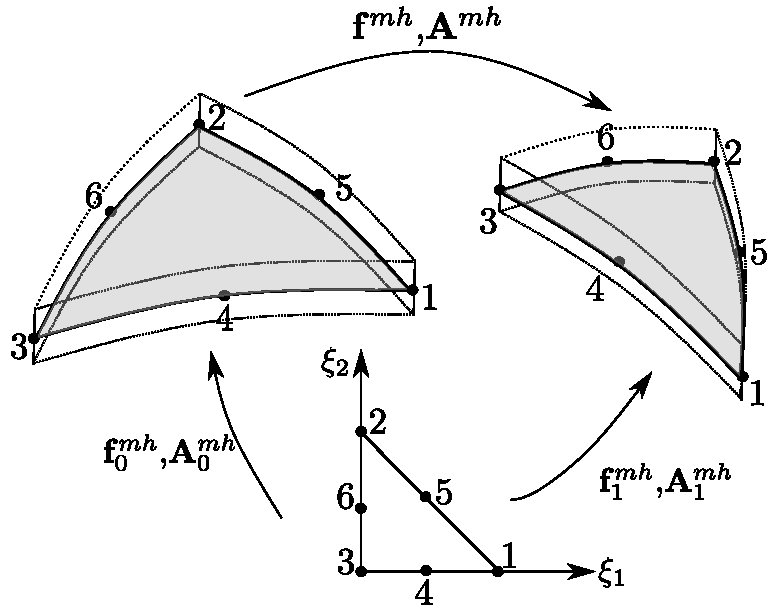
\includegraphics[scale=0.8,trim=0cm 0.0cm 0cm 0cm, clip=true]{Imagens/Cap4/casca_super_media.pdf}	
	\caption{Mapeamento da superfície média da casca}
	\label{fig:casca:map_super_media}
\end{figure}

Para completar a cinemática da casca, os demais pontos são mapeados por meio da soma da posição de um ponto na superfície média com um vetor generalizado $\mathbf{g}^{0h}$ ou $\mathbf{g}^{1h}$ nas configurações inicial e atual, respectivamente.  $\mathbf{g}^{0h}$ é normal a linha de referência na configuração inicial, conforme pode ser observado na Fig. \ref{fig:casca_vetores_generalizados}. Desta forma, o mapeamento completo fica definido por:

\begin{align}
\fmap^{0h}(\xi_{1},\xi_{2},\xi_{3}) = \lPosition^{h}(\xi_{1},\xi_{2},\xi_{3}) = \fmap^{0m}(\xi_{1},\xi_{2}) + \mathbf{g}^{0h} (\xi_{1},\xi_{2}, \xi_{3}) \label{eq:fmap0}\\
\fmap^{1h}(\xi_{1},\xi_{2},\xi_{3}) = \ePosition^{h}(\xi_{1},\xi_{2},\xi_{3}) = \fmap^{1m}(\xi_{1},\xi_{2}) + \mathbf{g}^{1h} (\xi_{1},\xi_{2}, \xi_{3})  \label{eq:fmap1}
\end{align}

\noindent em que $\xi_3$ é a coordenada adimensional na espessura da casca variando de -1 a 1.

\begin{figure}[htb!]
	\centering
	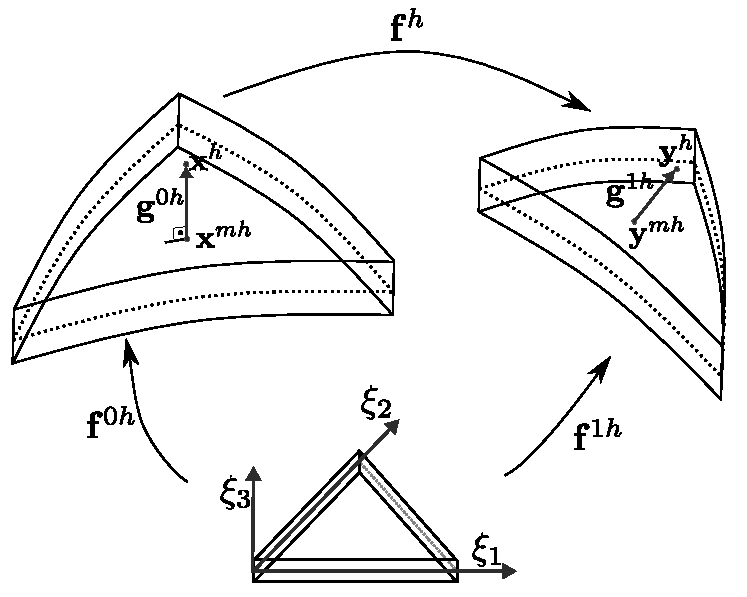
\includegraphics[scale=0.8,trim=0cm 0.0cm 0cm 0cm, clip=true]{Imagens/Cap4/casca_vetores_generalizados.pdf}	
	\caption{Vetores generalizados.}
	\label{fig:casca_vetores_generalizados}
\end{figure}

Os vetores generalizados $\mathbf{g}^{0h}$ e $\mathbf{g}^{1h}$ representados na discretização por elementos finitos ficam expressos por:

\begin{align}
\mathbf{g}^{0h} (\xi_{1},\xi_{2}, \xi_{3}) = \frac{h_{0}}{2}\xi_{3} N_{l}\left(\xi_{1},\xi_{2}\right) \cdot  (\mathbf{e}_x)_l, \\
\mathbf{g}^{1h} (\xi_{1},\xi_{2}, \xi_{3}) = \frac{h_{0}}{2}\left[\xi_{3} + \eta_l N_l\left(\xi_{1},\xi_{2}\right)\xi_{3}^2\right]N_{l}\left(\xi_{1},\xi_{2}\right) \cdot (\mathbf{e}_y)_l,
\end{align}

\noindent com $h_{0}$ representando a espessura média inicial do elemento de casca, $(\mathbf{e}_x)_l$ é o l-ésimo valor nodal do vetor unitário normal à linha de referência inicial, $(\mathbf{e}_y)_l$ o l-ésimo valor nodal do vetor generalizado na configuração atual e $\eta_l$ é o l-ésimo valor nodal da chamada de taxa linear de variação da espessura.

As equações Eq. \eqref{eq:fmap0} e Eq. \eqref{eq:fmap1} apresentam sete parâmetros incógnitos em cada nó $l$: 3 posições ($\ePosition_{l}^{mh}$), 3 componentes do vetor generalizado ($(\mathbf{e}_y)_l$) e o valor nodal da variação linear da deformação na espessura $\eta_l$. A partir desse ponto os parâmetros incógnitos serão descritos por uma única variável $ \SolidPos_{l}^{i}$, com $i = 0,1$ e $2$ representando as posições, $i = 3,4$ e $5$ as componentes do vetor generalizado e $i = 6$ a taxa de variação linear da espessura.

Para iniciar-se a descrição do MEF posicional, adiciona-se mais um termo à Eq. \eqref{eq:equi_local_forma_final} respectivo a forças concentradas nodais e fica-se com a seguinte definição para as equações de equilíbrio em descrição Lagrangiana:

\begin{align}
 -\mathbf{F}_{l}\delta\SolidPos_{l} - \int_{V_{0}}\bodyLoad \cdot \delta\ePosition dV_{0} - \int_{A_{0}} \ltractionLoad \cdot \delta\ePosition dA_{0} + \int_{V_{0}} \rho_{0} \solidAccel \cdot \delta\ePosition dV_{0} + \int_{V_{0}} \piolaStress : \delta\greenStrain dV_{0} = 0,
\end{align}

\noindent sendo o termo $\mathbf{F}_{l}$ respectivo a força concentrada aplicada sobre o nó $l$. O tensor $\greenStrain = \greenStrain (\SolidPos)$ é função de $\gradDeformation$, e pode ser obtido em função das posições através de $\fmap^{0h} $ e $\fmap^{1h} $ como:

\begin{align}
\gradDeformation = \gradDeformation^{1} \cdot \left(\gradDeformation^{0}\right)^{-1} \label{eq:gradDeformation}.
\end{align}

PAREI AQUI

Considerando uma aproximação tradicional das variáveis de elementos finitos, tem-se:

\begin{align}
\delta\ePosition = N_{l} (\xi_{1},\xi_{2})\delta\SolidPos_{l},\\
\bodyLoad = N_{l} (\xi_{1},\xi_{2}) \mathbf{B}_{l}^{0},\\
\ltractionLoad = N_{l} (\xi_{1},\xi_{2}) \mathbf{Q}_{l}^{0},\\
\solidAccel = N_{l} (\xi_{1},\xi_{2}) \mathbf{\ddot{Y}}_{l},
\end{align}

\noindent da arbitrariedade de $\delta\SolidPos$ as equações do equilíbrio em função das posições nodais são escritas como:

\begin{align}
\begin{split}
&-\mathbf{F}_{l} - \int_{V_{0}^{el}}N_{m} (\coordAdimen)N_{l} (\coordAdimen)dV_{0}^{el} \mathbf{B}_{m}^{0} -\int_{A_{0}^{el}}N_{m} (\coordAdimen)N_{l} (\coordAdimen)dA_{0}^{el} \mathbf{Q}_{m}^{0}  \\& + \int_{V_{0}^{el}}\rho_{0} N_{m} (\coordAdimen)N_{l} (\coordAdimen)dV_{0}^{el} \mathbf{\ddot{Y}}_{m} + \int_{V_{0}^{el}} \piolaStress : \frac{\partial\greenStrain}{\partial\SolidPos_{l}}dV_{0}^{el}.
\end{split}
\end{align}

%\subsection{Integração temporal e técnica de solução}
%
%As equações do equilíbrio baseadas em posição podem ser apresentadas sinteticamente como:
%
%\begin{align}
%\frac{\partial\totalEnergy}{\partial\SolidPos} = \frac{\partial\extEnergy}{\partial \SolidPos} + \frac{\partial\kinEnergy}{\partial \SolidPos} + \frac{\partial\intEnergy}{\partial \SolidPos} = \mathbf{0},
%\end{align}
%  
%\noindent ou ainda,
%
%\begin{align}
% - \concLoad^{ext}(t) + \solidMass\SolidAccel_{}+ \concLoad^{int}(\SolidPos) + \solidDamping\SolidVel_{} = \mathbf{0}, \label{eq:Equilibrio}
%\end{align}
%
%\noindent na qual $ \concLoad^{int}(\SolidPos)$ representa as forças internas provenientes da variação da energia potencial interna, $\solidMass$ é a conhecida como matriz de massa proveniente da variação da energia cinética e $\mathbf{F}^{ext}$ representam as forças externas na estrutura fruto da variação da energia potencial das forças externas. O termo $\solidDamping$ representa uma matriz de amortecimento proporcional a massa, e $\SolidVel_{}$ a velocidade nodal.
%
%A integração temporal das equações apresentadas na Eq. \eqref{eq:Equilibrio} inicia-se com a discretização temporal do tempo de maneira que:
%
%\begin{align}
%t_{n+1} = t_{n} + \Delta t, \label{eq:disTime}
%\end{align}
%
%\noindent na qual $t_{n+1}$ representa o tempo no instante atual, $t_{n}$ o instante de tempo anterior e  $\Delta t$ o intervalo de tempo utilizado na discretização. Utilizando as aproximações de Newmark, posições, velocidade e aceleração nos tempos $n+1$ e $n$ são relacionados por:
%
%\begin{gather}
%\SolidPos_{n+1}=\SolidPos_{n} + \timeStep \SolidVel_{n}+\left(\frac{1}{2}-\beta\right) \timeStep^2 \SolidAccel_{n}+ \beta \timeStep^2 \SolidAccel_{n+1},\label{eq:newmark1}\\
%\SolidVel_{n+1} = \SolidVel_{n}+(1-\gamma)\timeStep \SolidAccel_{n}+\gamma \timeStep \SolidAccel_{n+1},\label{eq:newmark2}
%\end{gather}
%
%\noindent em que $\beta$ e $\gamma$ são parâmetros dependentes do comportamento assumido para a aceleração, adotados nesse trabalho como $\gamma=\sfrac{1}{2}$ e $\beta=\sfrac{1}{4}$ para uma aceleração constante.
%
%Considerando a discretização temporal apresentada em Eq. \eqref{eq:disTime} e aplicando-se a Eq. \eqref{eq:newmark1} e Eq. \eqref{eq:newmark2} à Eq. \eqref{eq:Equilibrio} de maneira a escrever-se a equação somente em função das posições nodais, tem-se, para um instante $n+1$ a seguinte relação:
%
%\begin{gather}
%\concLoad^{int}_{n+1}- \concLoad^{ext}_{n+1} + \frac{\solidMass}{\beta \timeStep^2} \SolidPos_{n+1}-\solidMass \mathbf{Q}_n+ \solidDamping\mathbf{R}_n + \frac{\gamma \solidDamping}{\beta \timeStep}\SolidPos_{n+1} - \gamma\timeStep \solidDamping\mathbf{Q}_n = \mathbf{0},
%\label{eq:equilibrio_newmark}
%\end{gather}
%
%\noindent em que $\mathbf{Q}_n$ e $\mathbf{R}_n$ representam os termos dependentes apenas de velocidades, acelerações e posições do instante anterior, dados por:
%
%\begin{gather}
%\mathbf{Q}_n = \frac{\SolidPos_n}{\beta \timeStep^2} + \frac{\SolidVel_n}{\beta \timeStep} + \left(\frac{1}{2\beta} -1 \right)\SolidAccel_n,\label{eq:Qn}\\
%\mathbf{R}_n = \SolidVel_n+\timeStep(1-\gamma)\SolidAccel_n.\label{eq:Rn}
%\end{gather}
%
%
%Pode-se escrever ainda o problema não linear definido por
%\eqref{eq:equilibrio_newmark} em função do resíduo da equação governante
%discretizada no espaço e no tempo, tal que:
%
%%\begin{gather}
%%%\begin{dcases}
%%\NNSS\left(\SolidPos_{n+1}\right) = \concLoad^{int}_{n+1}- \concLoad^{ext}_{n+1} + \frac{\solidMass}{\beta \timeStep^2} \SolidPos_{n+1}-\solidMass \mathbf{Q}_n+ \solidDamping\mathbf{R}_n + \frac{\gamma \solidDamping}{\beta \timeStep}\SolidPos_{n+1} - \gamma\timeStep \solidDamping\mathbf{Q}_n= \zeroMatrix.
%%%\end{dcases}
%%\label{eq:equilibrio_newmark1.5}
%%\end{gather}
%
%O problema não linear da Eq. \eqref{eq:equilibrio_newmark1.5} é resolvido por meio do método iterativo de Newton-Raphson. Para isso, realiza-se uma expansão em série de Taylor de primeira ordem:
%
%\begin{gather}
%\NNSS\left(\SolidPos_{n+1}^{i+1}\right) \approx \NNSS\left(\SolidPos_{n+1}^{i}\right) + \Delta\NNSS\left(\SolidPos_{n+1}^{i}\right)\Delta\SolidPos_{i} 
%\end{gather}
%
%\noindent em que $i$ indica o índice da iteração atual. Na primeira iteração para o cálculo de $\SolidPos_{n+1}$ utiliza-se como predição da iteração anterior os valores das variáveis no passo de tempo $n$. O método de Newton-Raphson consiste em resolver o seguinte sistema:
%
%\begin{gather}
%\Delta\NNSS\left(\SolidPos_{n+1}^{i}\right)\Delta\SolidPos^{i} = -\NNSS\left(\SolidPos_{n+1}^{i}\right) \label{eq:NR}
%\end{gather}
%
%\noindent com:
%
%\begin{gather}
%\Delta\NNSS\left(\SolidPos_{n+1}^{i}\right) = \frac{\partial^{2}\totalEnergy}{\partial\SolidPos^{2}} = \frac{\partial^{2}\intEnergy}{\partial \SolidPos^{2}} + \frac{\solidMass}{\beta \timeStep^2} + \frac{\gamma \solidDamping}{\beta \timeStep}.
%\end{gather}
%
%A cada iteração de Newton-Raphson atualiza-se a posição, a aceleração e a velocidade de acordo com as seguintes equações:
%
%\begin{gather}
%\SolidPos_{n+1}^{i+1} = \SolidPos_{n+1}^{i} + \Delta\SolidPos^{i} \label{UD1}\\
%\SolidAccel_{n+1}^{i+1} = \frac{\SolidPos_{n+1}^{i+1}}{\beta \timeStep^2} + \mathbf{Q}_n  \label{UD2} \\
%\SolidVel_{n+1}^{i+1} = \frac{\gamma \SolidPos_{n+1}^{i+1}}{\beta \timeStep} + \mathbf{R}_n - \gamma\Delta t \mathbf{Q}_n  \label{UD3}
%\end{gather}
%
%
%\subsection{Implementação Computacional}
%
%Emprega-se o programa para análise não linear de estruturas de casca cedido pelo professor Humberto Breves Coda \cite{CodaP:2007,CodaP:2008}, o qual segue a formulação descrita neste texto e é implementado em linguagem FORTRAN, com paralelização em protocolo MPI.
%
%O algoritmo implementado foi criteriosamente estudado de forma a permitir a implementação do acoplamento, sendo apresentado em Alg. \ref{alg:solid_temporalIntegration}.
%
%
%\begin{algorithm}
%	\caption{Algoritmo para problemas de dinâmica dos sólidos computacional}
%	\label{alg:solid_temporalIntegration}
%	\begin{algorithmic}[1]
%		\For {o passo de tempo $0$ até MUDAR TEMPO} 
%		\State $i=0$;
%		\State Predição da solução: 
%		\begin{align}
%		\SolidPos_{n+1}^{0} = \SolidPos_{n},\\
%		\SolidVel_{n+1}^{0} = \SolidVel_{n},\\
%		\SolidAccel_{n+1}^{0} = \SolidAccel_{n};
%		\end{align}
%		\State Calcula-se  nível de força aplicado $\concLoad^{ext}_{n+1}(t_{n+1})$ e/ou as posições prescritas $\SolidPos_{n+1}$;
%		\State Calculam-se os valores de $\mathbf{Q}_n$ (Eq. \eqref{eq:Qn}) e $\mathbf{R}_n$ (Eq. \eqref{eq:Rn});
%		\While{($\epsilon$ < tolerância)}
%		\State $i$++;
%		\State Cálculo do incremento da variável do problema: $\SolidPos_{n+1}^{i}$ de acordo com a Eq. \eqref{eq:NR};
%		\State Atualização da solução: calculada de acordo com Eq. \eqref{UD1}, Eq. \eqref{UD2} e Eq. \eqref{UD3}.
%		\State Cálculo do erro:
%		\begin{align}
%		\epsilon = \lVert \Delta\NNSS\left(\SolidPos_{n+1}^{i+1}\right) \lVert_{L^2} 
%		\end{align}
%		ou,
%		\begin{align}
%		\epsilon = \lVert\Delta\SolidPos_{n+1}^{i+1}\lVert_{L^2} 
%		\end{align}
%		\EndWhile
%		\EndFor
%	\end{algorithmic}
%\end{algorithm}
%
%\section{Exemplo de aplicação - Casca cilíndrica com \textit{snap through} dinâmico}
%
%Nesta seção é apresentada uma simulação feita com o código cedido pelo professor Humberto Breves Coda para problemas de análise não-linear geométrica de cascas. Esta análise foi realizada com o objetivo de estudar o programa a ser empregado na pesquisa.
%
%O problema clássico analisado trata-se de um casca cilíndrica submetida a um carregamento concentrado em seu centro geométrico. Proposto inicialmente no trabalho de \cite{KuhlR:1999}, o problema apresenta grande não-linearidade geométrica devido ao efeito de \textit{snap-through}. 
%
%A geometria do problema em questão é apresentada na Fig. \ref{fig:CascaGeo}, sendo a espessura da casca equivalente a 0,1 m. Como condições de contorno, têm-se o deslocamento restrito nas direções $x,y,z$ para as bordas retas que formam a geometria da casca. A malha de elementos finitos que representa a superfície média da casca utilizada pode ser visualizada na Fig. \ref{fig:CascaMalha}, a qual é composta por 32 elementos cúbicos e 49 nós. 
%
%\begin{figure}[!htb]
%	\centering
%	\subfloat[\label{fig:CascaGeo} Malha Local.]{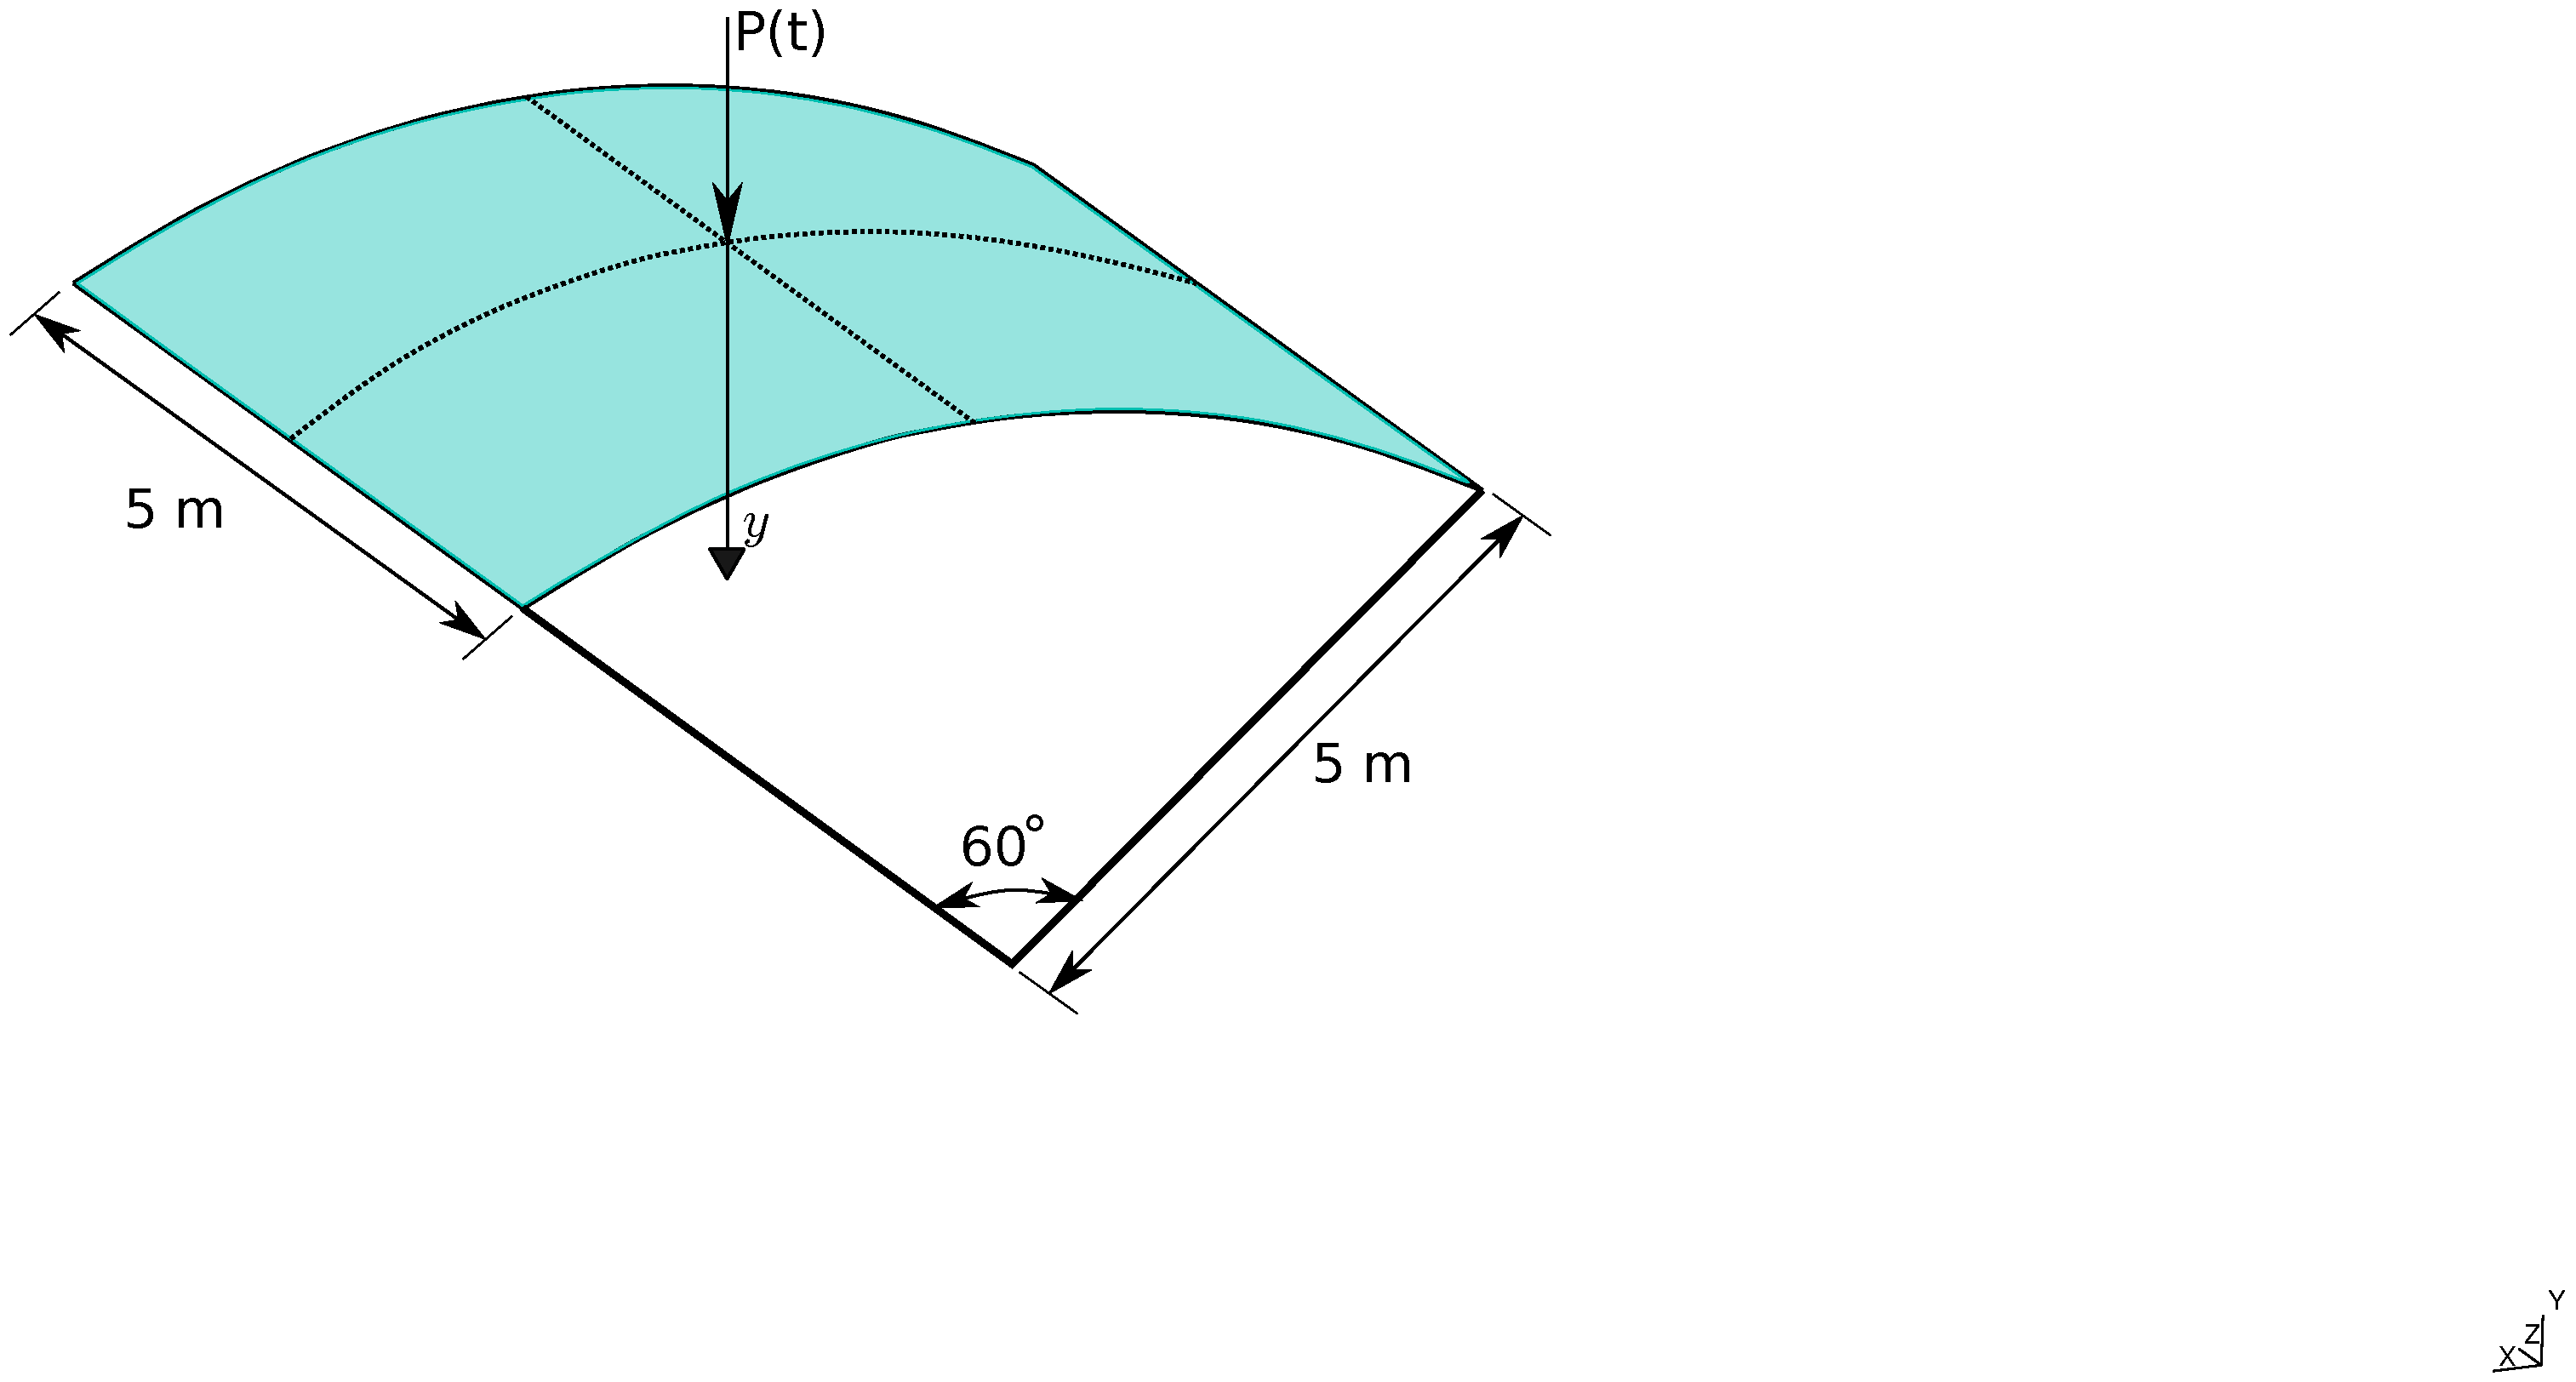
\includegraphics[scale=0.2, trim=0cm 0cm 15cm 0cm, clip=true]{Imagens/Cap4/lateral.pdf}} 
%	\subfloat[\label{fig:CascaMalha} Malha Global ]{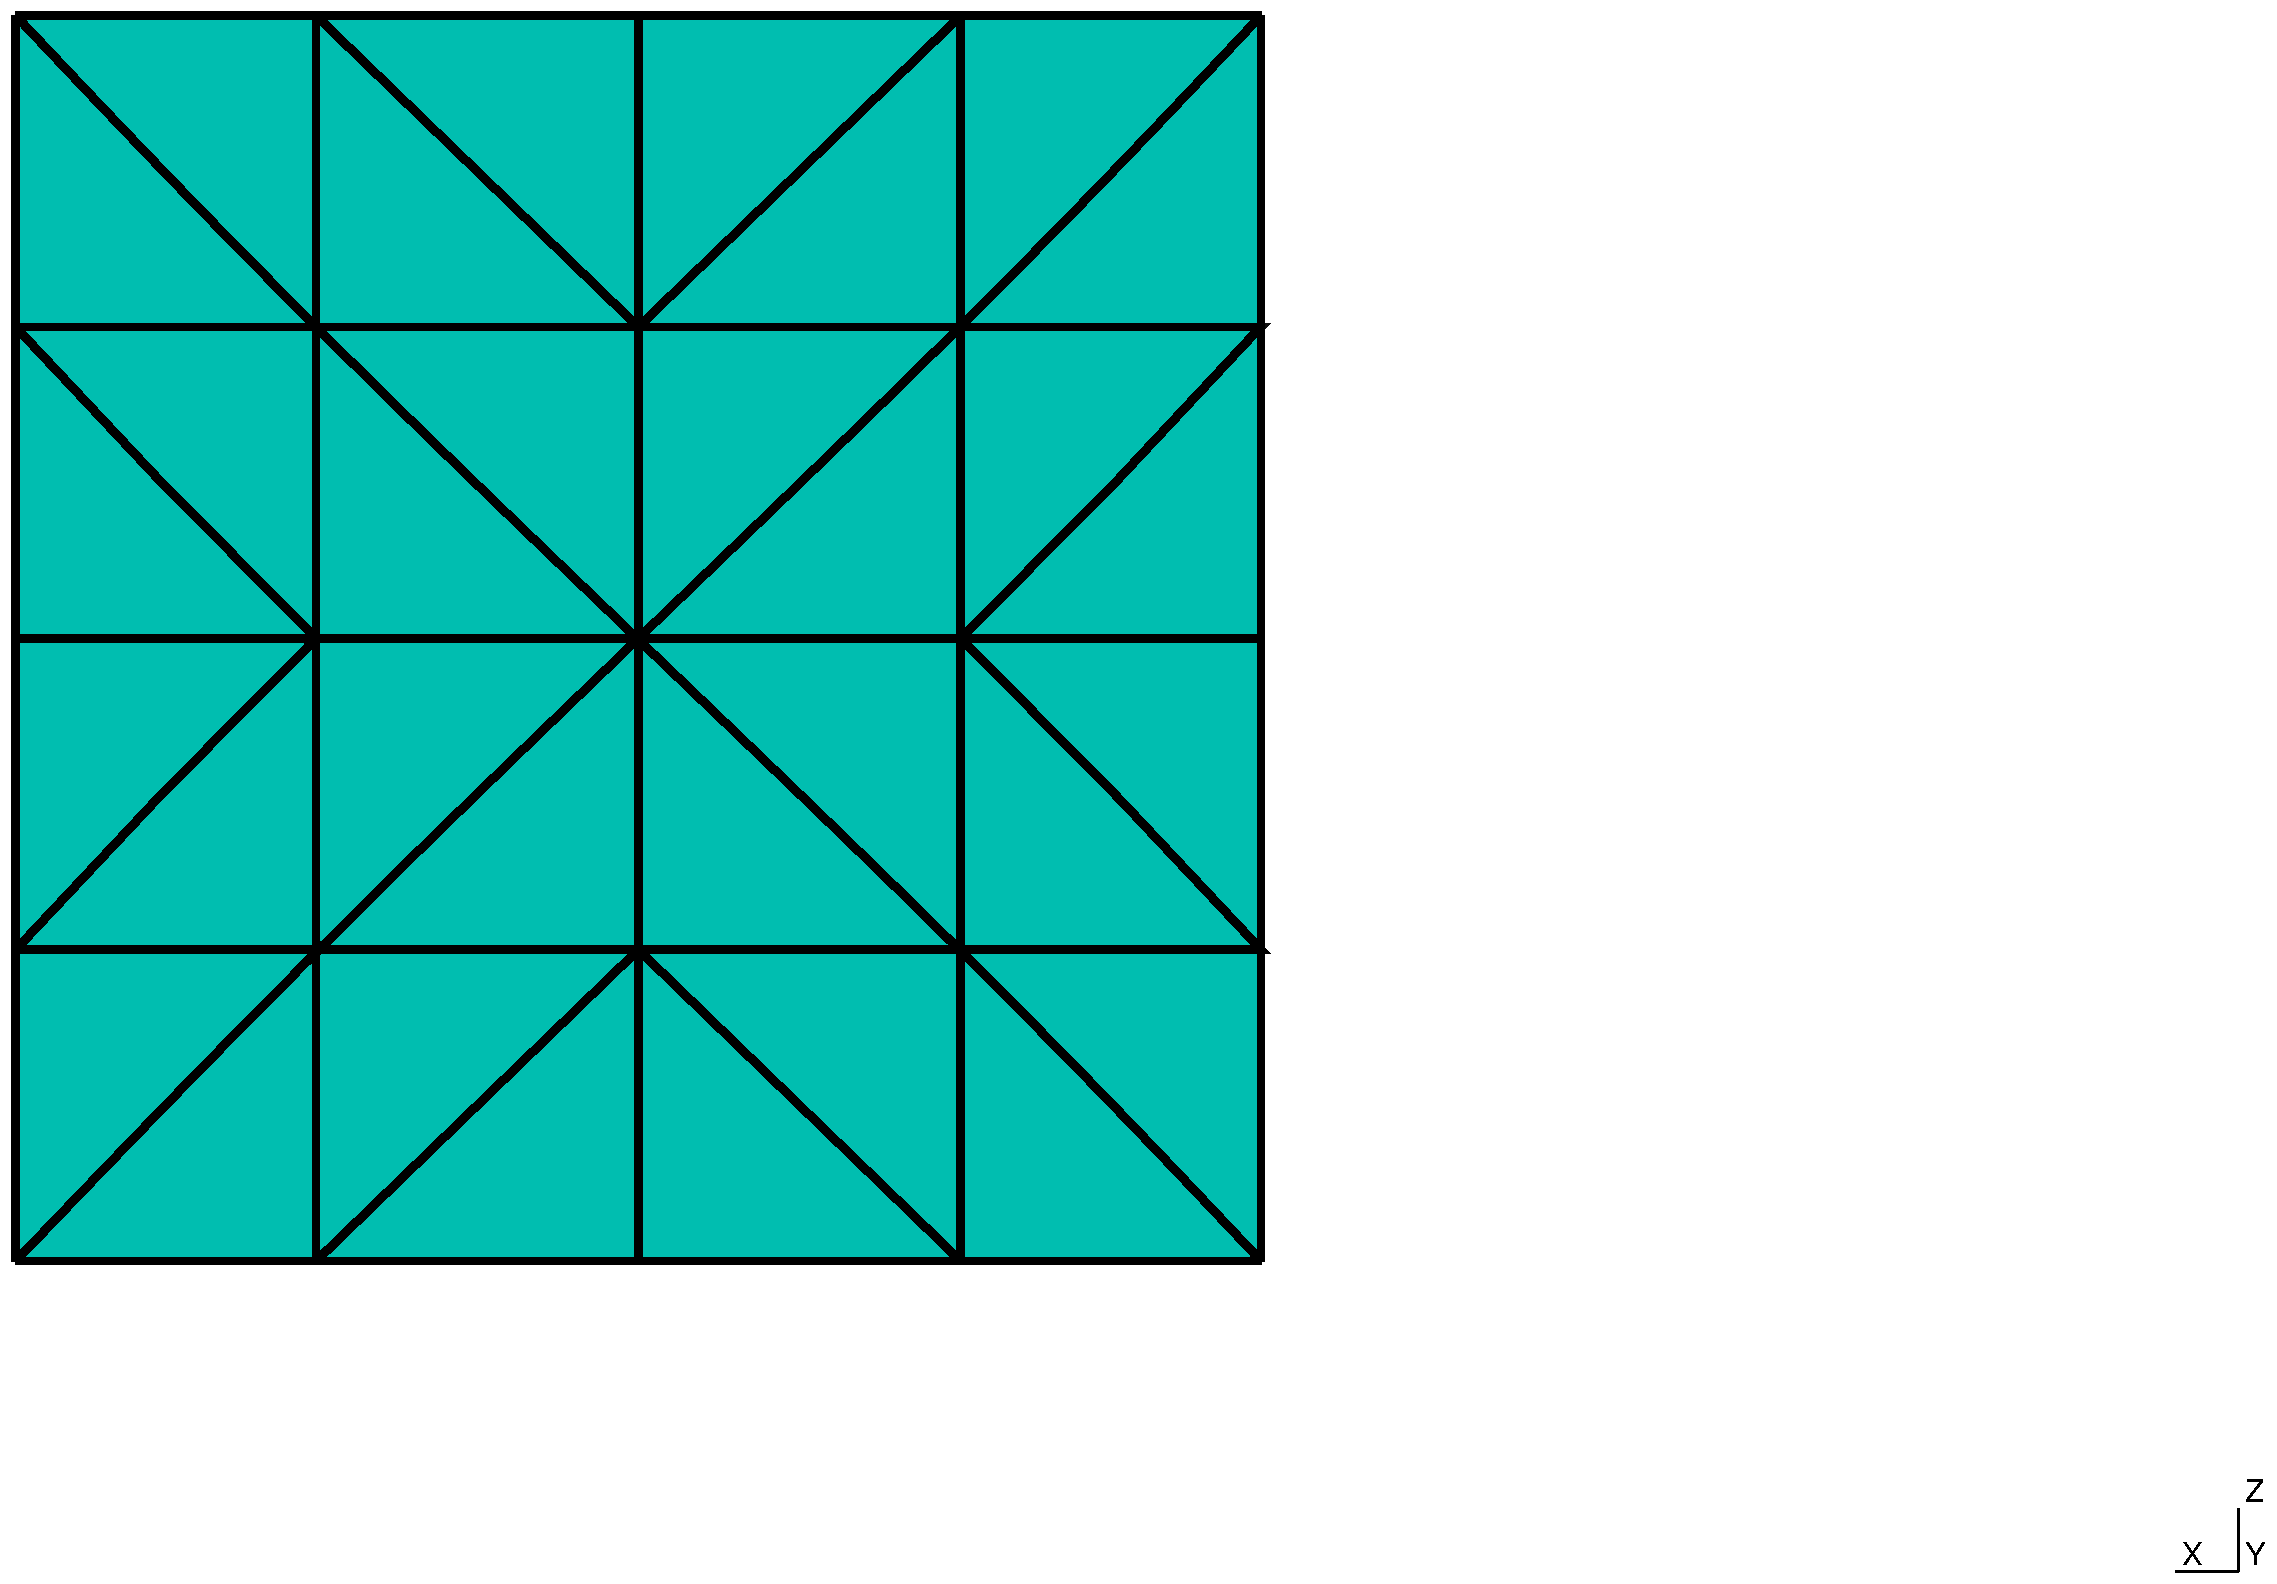
\includegraphics[scale=0.18,trim=0cm 0cm 15cm 0cm, clip=true]{Imagens/Cap4/teste.pdf}}
%	\caption{Casca: Geometria e Malha.}
%	\label{fig:Casca}
%\end{figure}
%
%O carregamento $P(t)$ é aplicado linearmente no intervalo $t=0s$ até $t=0,2s$, com $P(0)=0kN$ e $P(2s) = 50000kN$, e então mantido constante. As características físicas do material utilizado são: $\elasticModulus = 200GPa$, $\poisonsRatio = 0,25$ e $\rho = 10000 kg/m^3$ e o passo de tempo adotado na simulação é $\Delta_{t} = 0,001s$.
%
%O deslocamento vertical do nó central da casca pode ser visualizado na Fig. \ref{fig:CascaDeslocamento}. O resultado obtido está de acordo com os resultados de \citeonline{ArgyrisPM:2003}, conforme pode ser visto na Fig. \ref{fig:CascaDeslocamentoReferencia} e o campo de deslocamentos nos instantes $t = 0s$, $t = 100ms$ e $t = 155ms$ são apresentados na Fig. \ref{fig:CamposDeslocamentos}.
%
%Embora a implementação do programa de cascas não seja objetivo deste trabalho, e essa análise tenha objetivo de estudar o código a ser empregado, ela também traz indício da robustez e precisão da formulação escolhida.
%
%\begin{figure}[!htb]
%	\centering
%	\subfloat[\label{fig:CascaDeslocamento} Presente trabalho.]{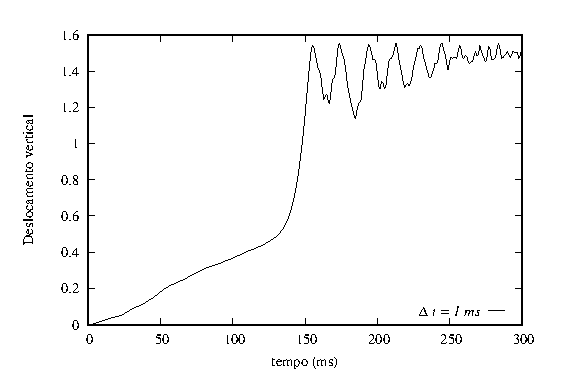
\includegraphics[scale=.8, trim=0cm 0cm 0cm 0cm, clip=true]{Imagens/Cap4/snap_casca.eps}} \\
%	\subfloat[\label{fig:CascaDeslocamentoReferencia} Referência ]{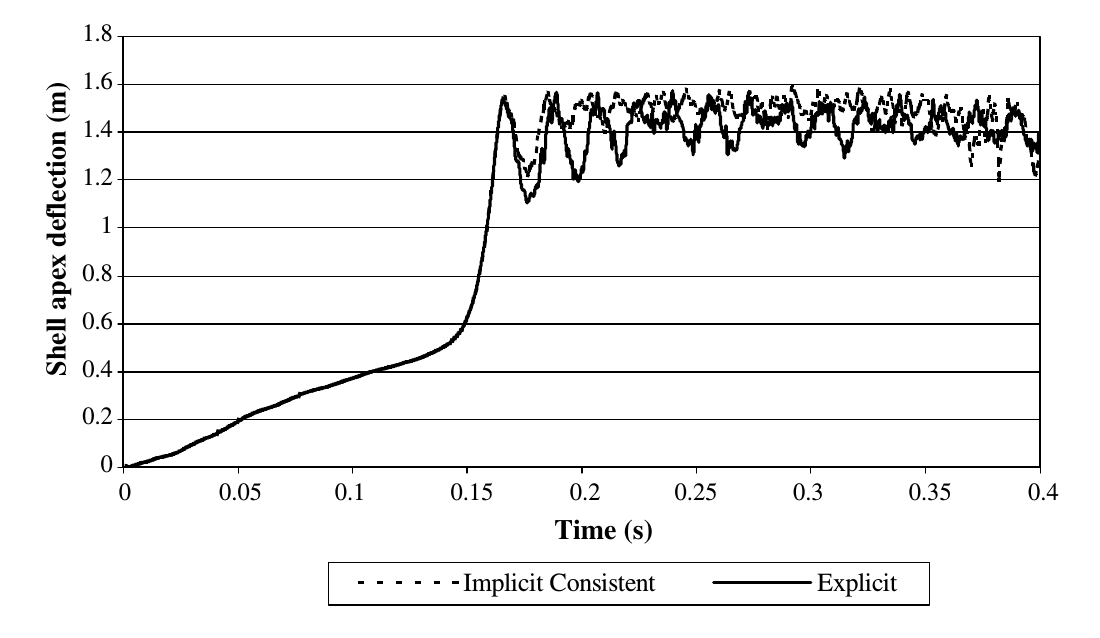
\includegraphics[scale=0.25,trim=0cm 0cm 0cm 0cm, clip=true]{Imagens/Cap4/referencia.png}}\\
%	Fonte: \citeonline{ArgyrisPM:2003}
%	\caption{Casca: Deslocamento vertical nó central.}
%	\label{fig:CascaDeslocamentoT}
%\end{figure}
%
%
%\begin{figure}[!htb]
%	\centering
%	\subfloat[\label{fig:C0} $t = 0s$.]{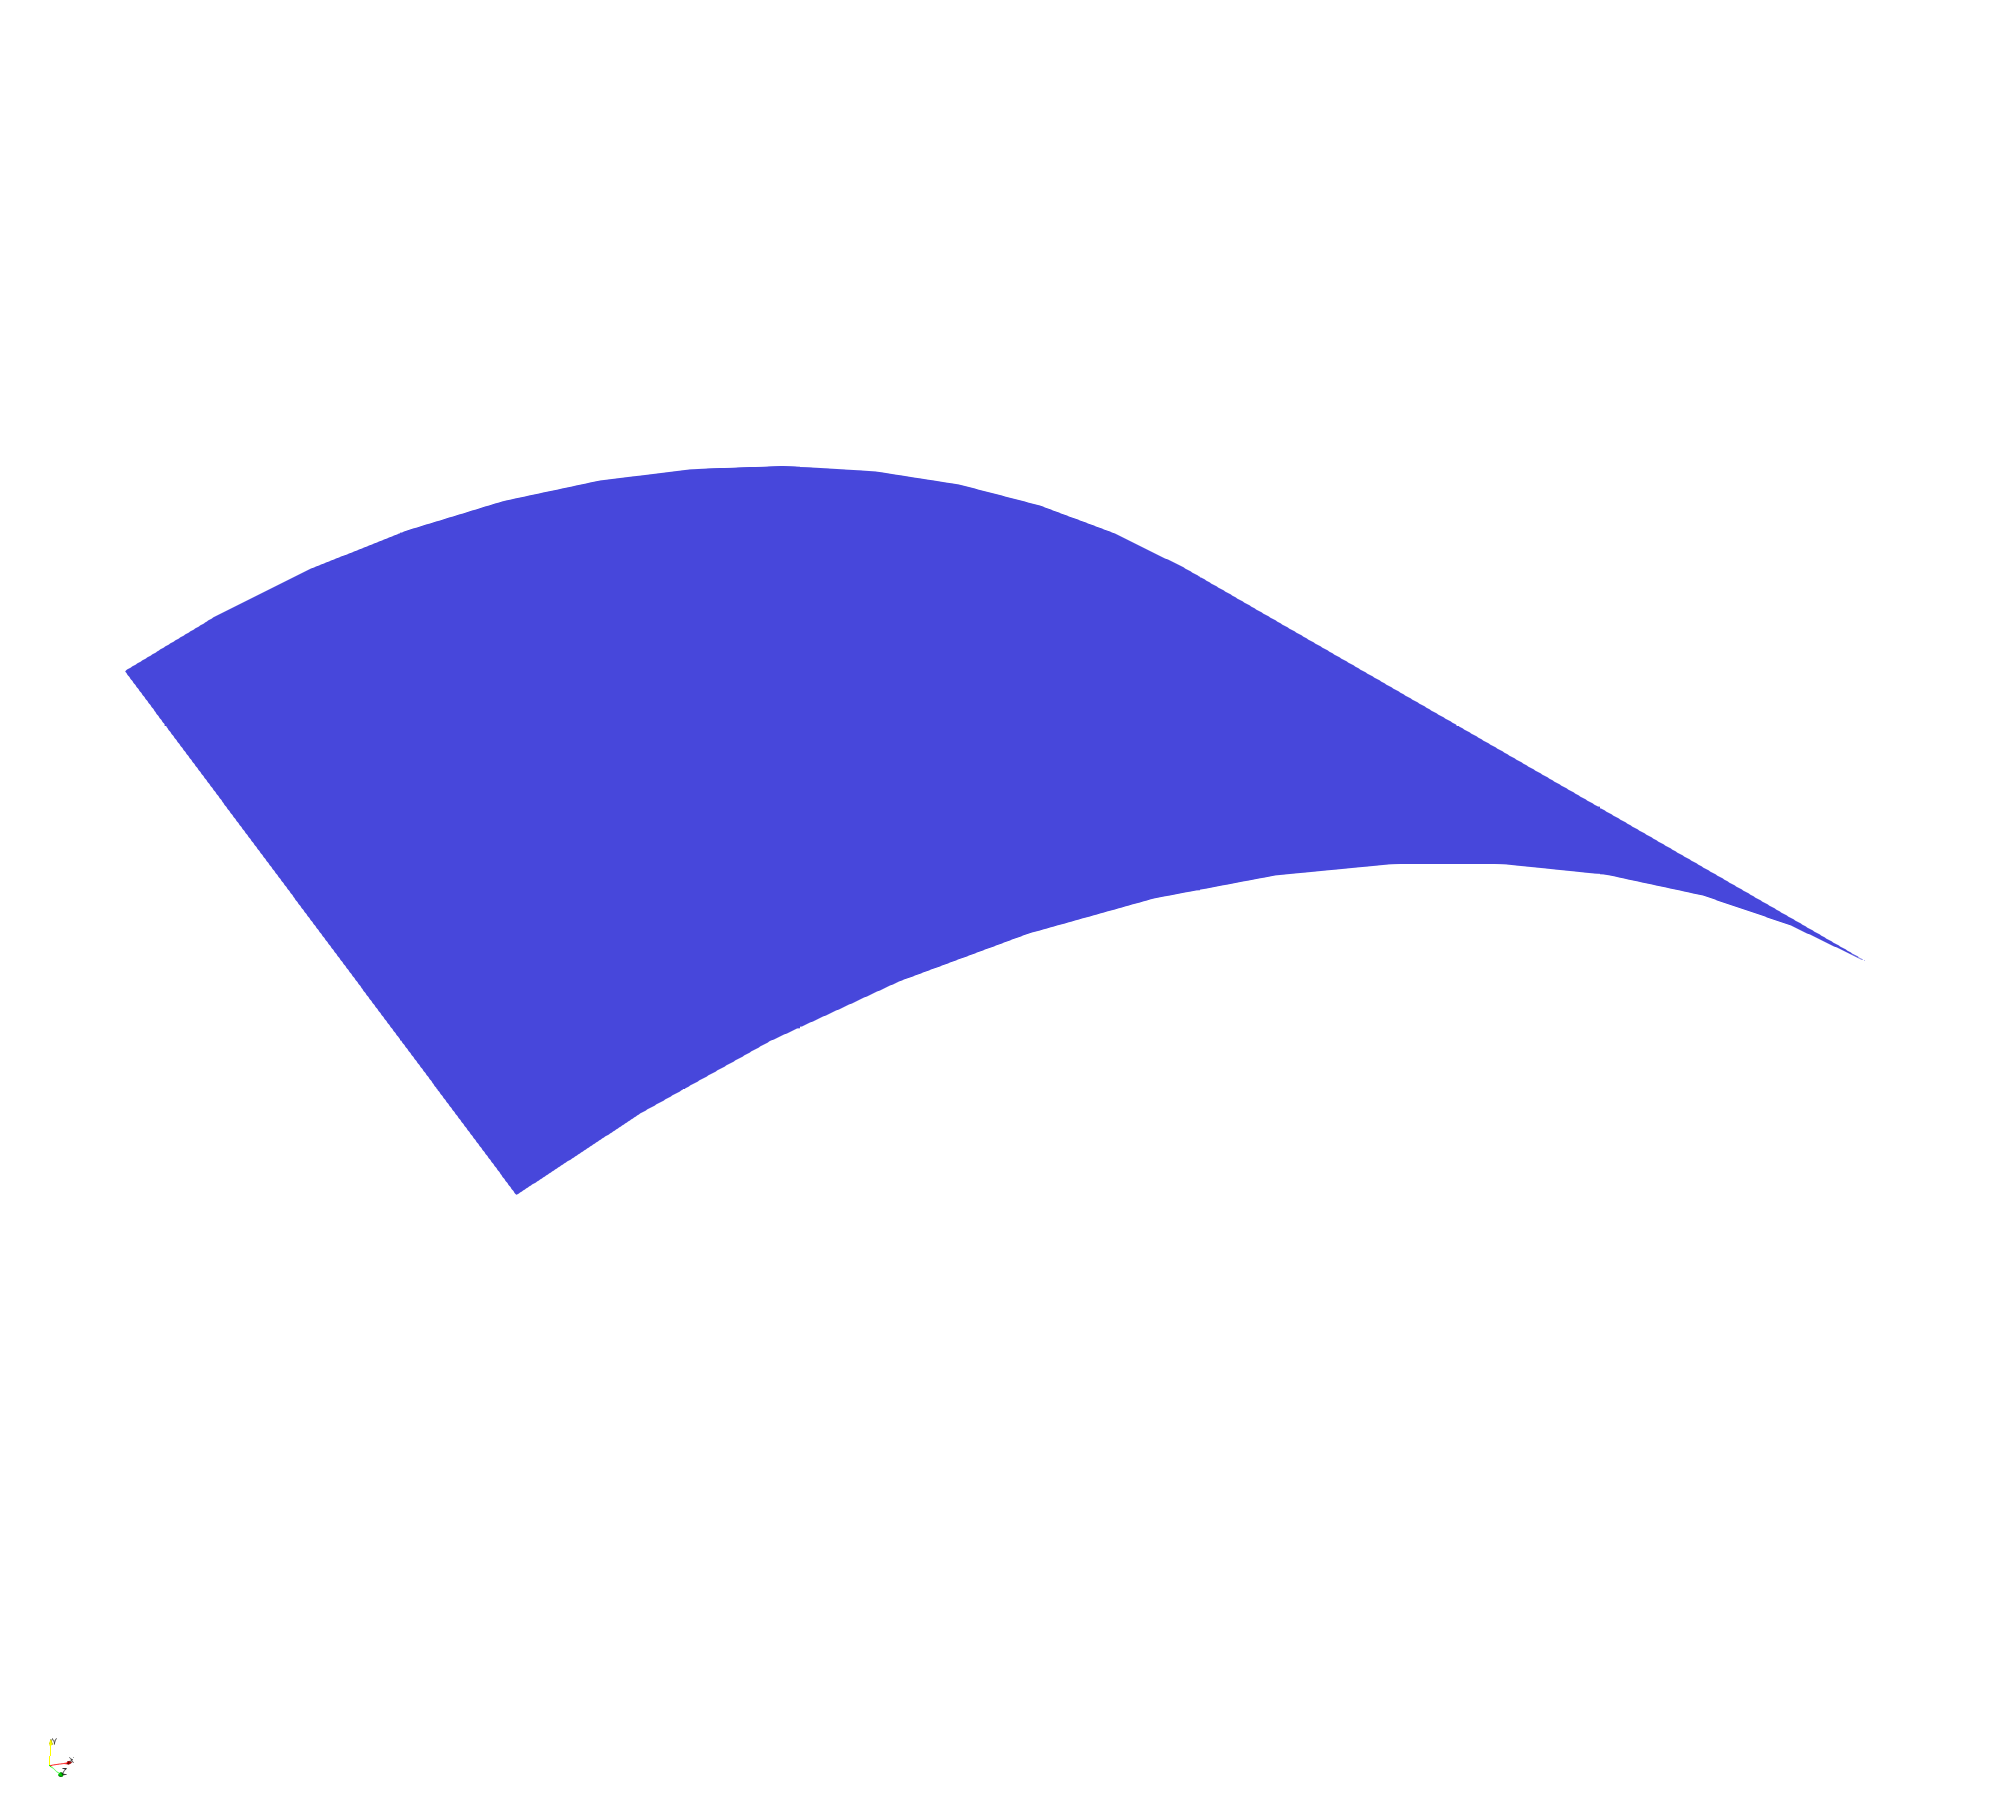
\includegraphics[scale=0.08, trim=4cm 15cm 4cm 15cm, clip=true]{Imagens/Cap4/0ms.png}} 
%	\subfloat[\label{fig:C1} $t = 100ms$ ]{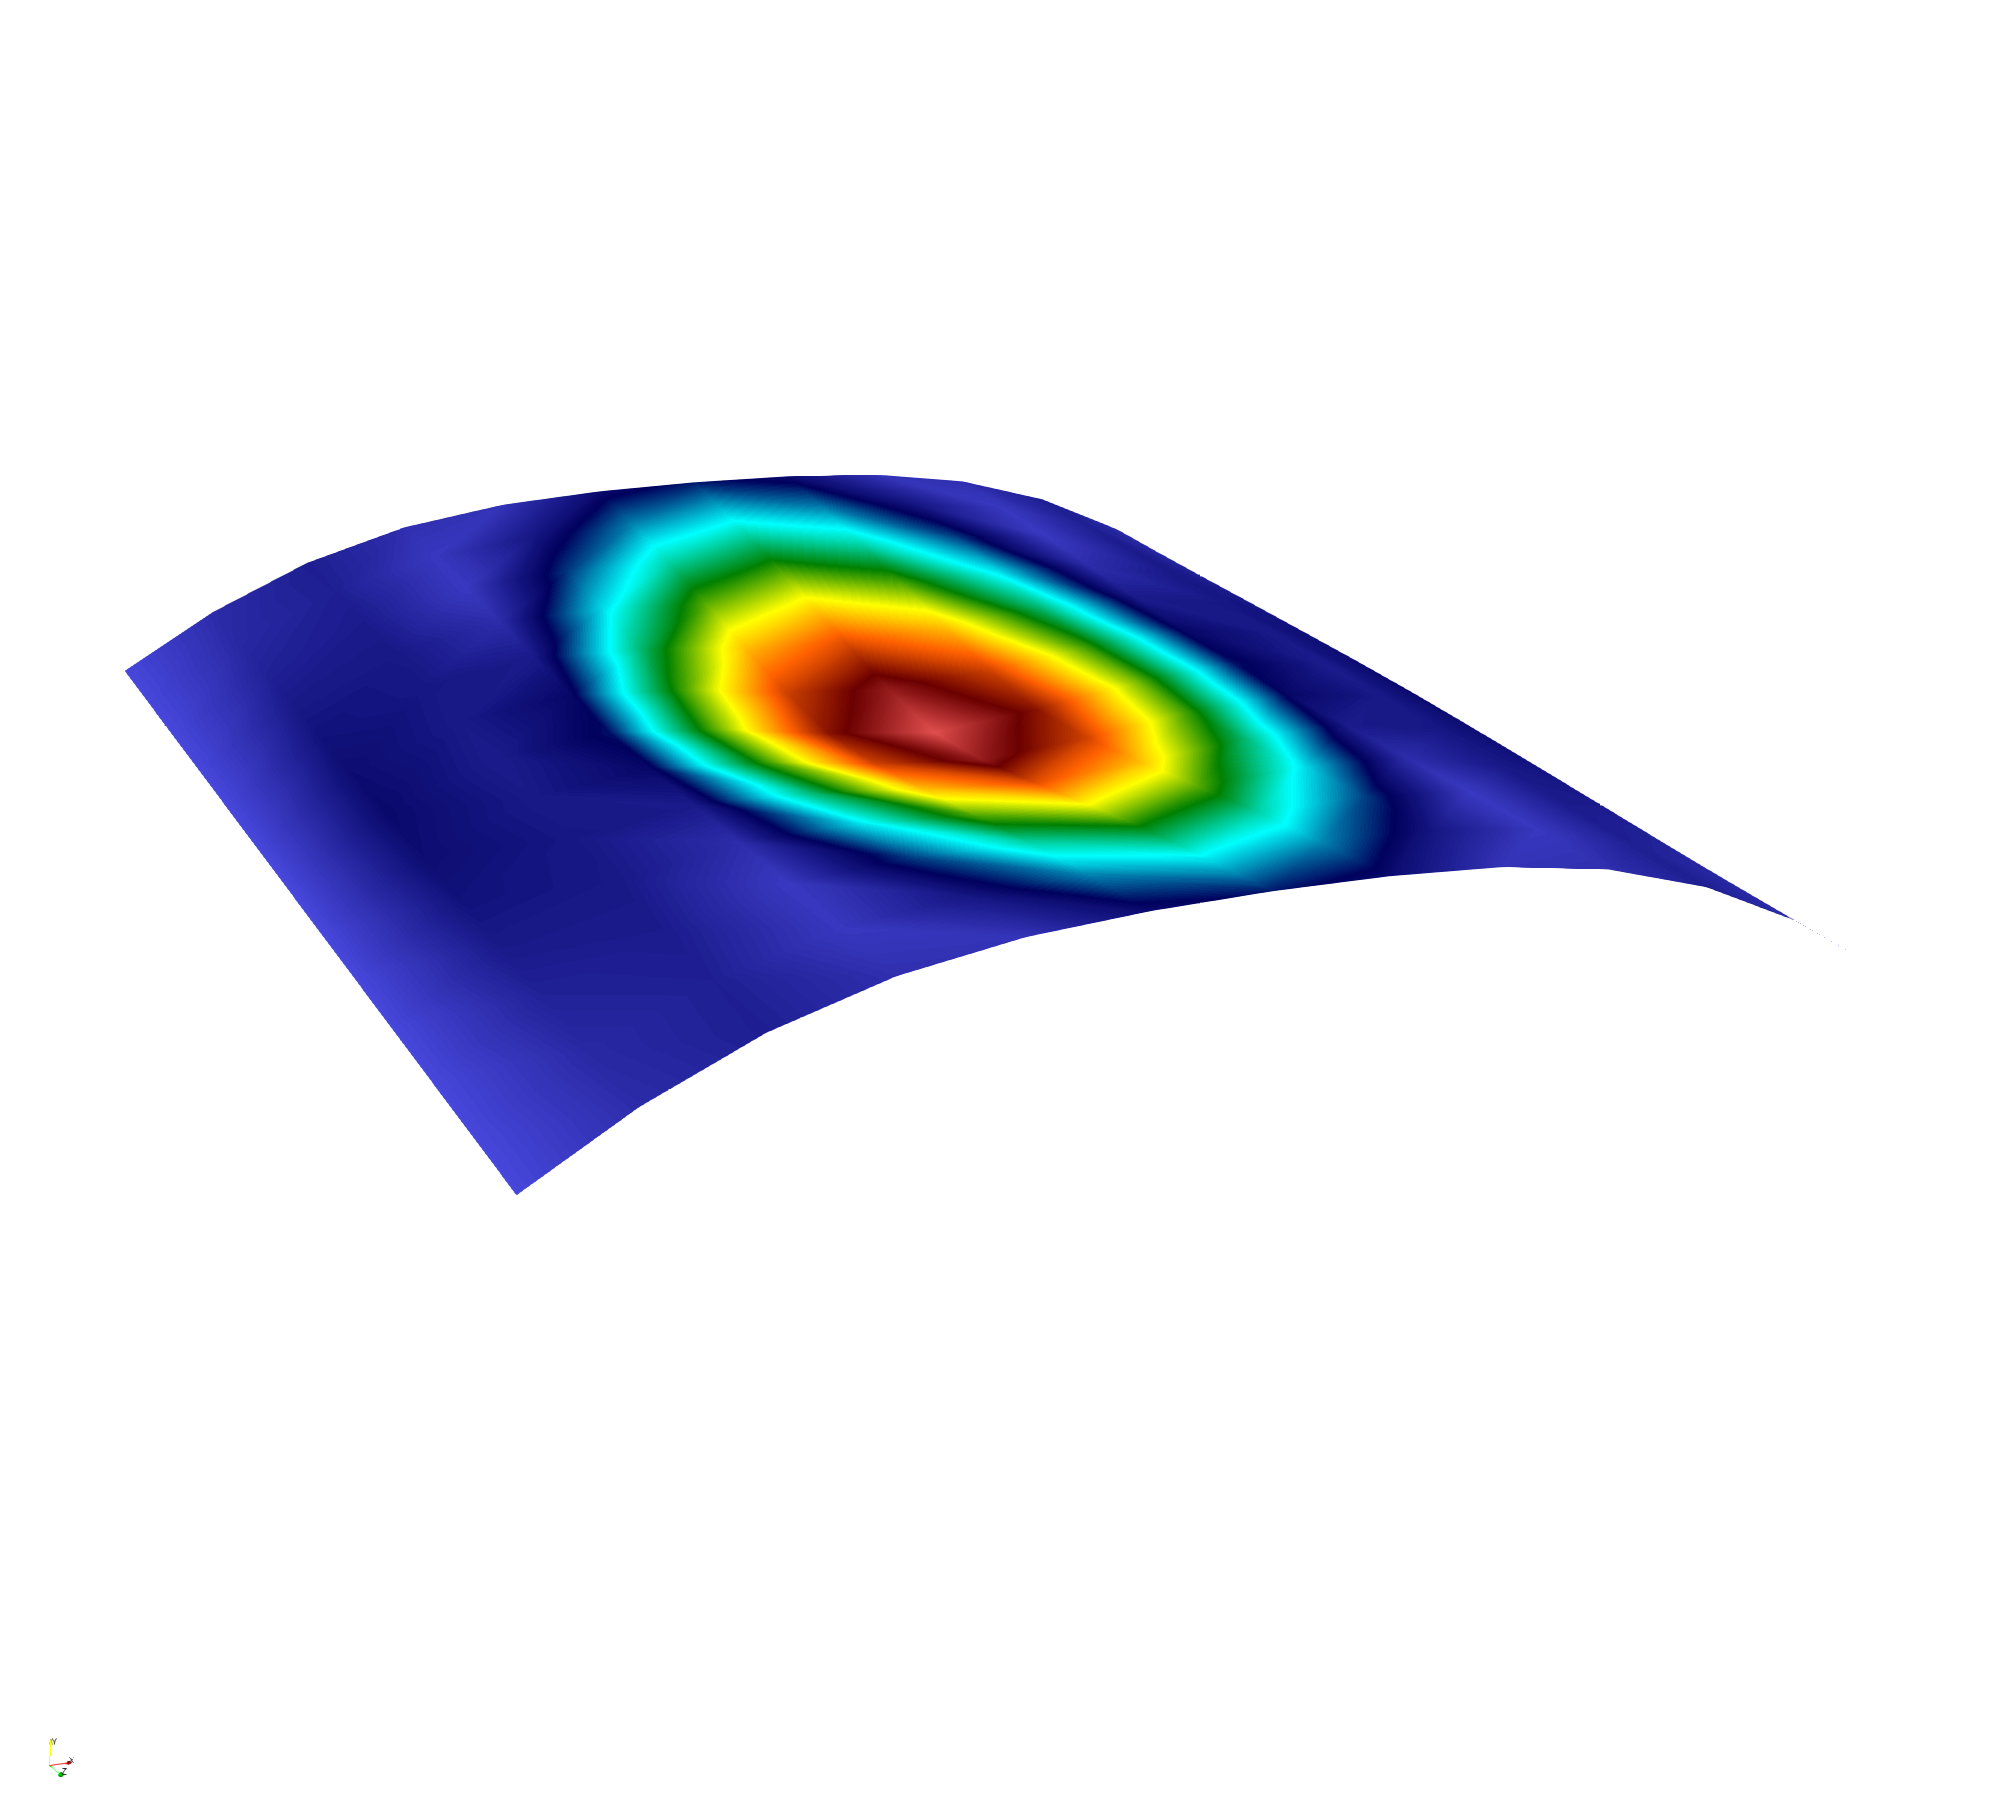
\includegraphics[scale=0.08,trim=4cm 15cm 4cm 15cm, clip=true]{Imagens/Cap4/100ms.png}}\\
%	\subfloat[\label{fig:C2} $t = 155ms$ ]{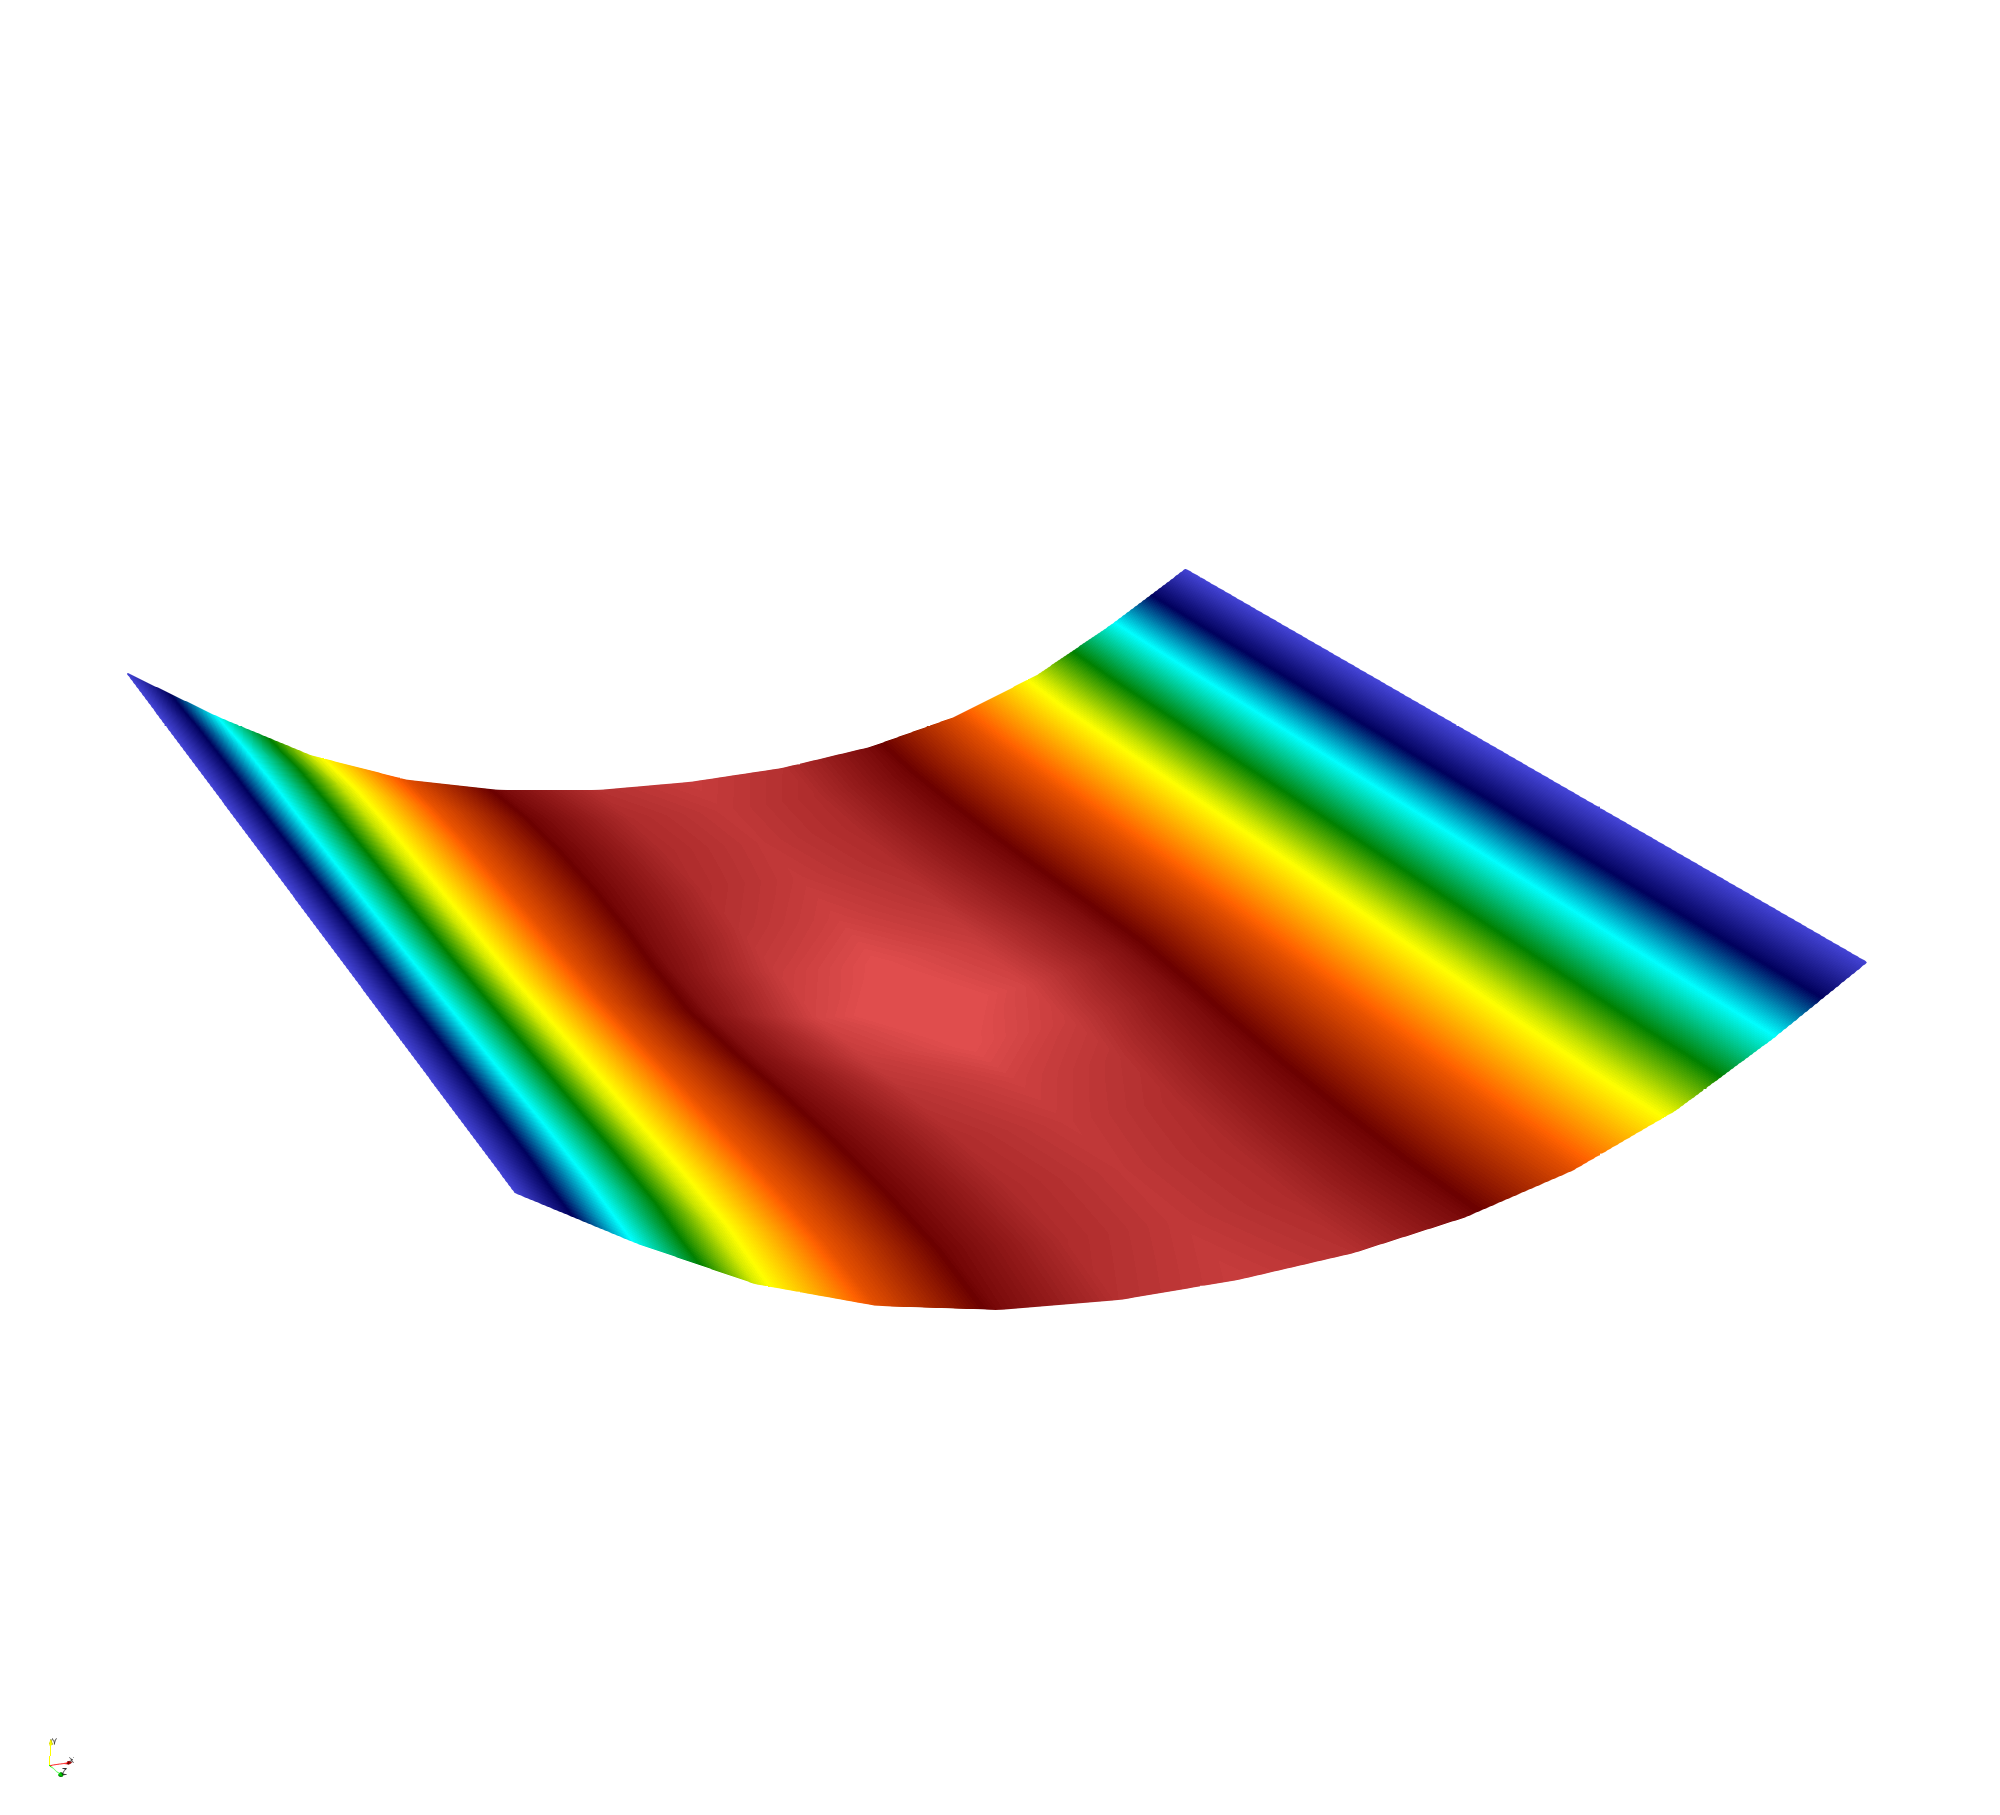
\includegraphics[scale=0.08,trim=4cm 15cm 4cm 15cm, clip=true]{Imagens/Cap4/155ms.png}}\\
%	{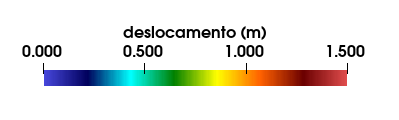
\includegraphics[scale=0.3,trim=0cm 0cm 0cm 0cm, clip=true]{Imagens/Cap4/legenda.png}}
%	\caption{Casca: Campo de deslocamento.}
%	\label{fig:CamposDeslocamentos}
%\end{figure}
%
%
%
%
%% \section{Validação e aplicações}
%%\textcolor{red}{voltamos a esse ponto se houver tempo...}
%% \subsection {Exemplo}

\end{document}